%
% Template Laporan Skripsi/Thesis 
%
% @author  Andreas Febrian, Lia Sadita 
% @version 1.03
%
% Dokumen ini dibuat berdasarkan standar IEEE dalam membuat class untuk 
% LaTeX dan konfigurasi LaTeX yang digunakan Fahrurrozi Rahman ketika 
% membuat laporan skripsi. Konfigurasi yang lama telah disesuaikan dengan 
% aturan penulisan thesis yang dikeluarkan UI pada tahun 2008.
%

%
% Tipe dokumen adalah report dengan satu kolom. 
%
\documentclass[12pt, a4paper, onecolumn, oneside, final]{report}

% Load konfigurasi LaTeX untuk tipe laporan thesis
\usepackage{uithesis}
\usepackage{natbib}
\usepackage{import}
\usepackage{enumitem}
\usepackage{adjustbox}
\usepackage{graphicx}
\usepackage{amsmath}
\usepackage{multirow}
\usepackage{pdfpages}
\usepackage{pdflscape}
% Load konfigurasi khusus untuk laporan yang sedang dibuat
%-----------------------------------------------------------------------------%
% Informasi Mengenai Dokumen
%-----------------------------------------------------------------------------%
% 
% Judul laporan. 
\var{\judul}{Pengembangan \f{Prototype} Hasil Analisis Aspek \f{Usability Website E-Government}: Studi Kasus \f{Website} Direktorat Jenderal Pajak Indonesia dengan India}
% 
% Tulis kembali judul laporan, kali ini akan diubah menjadi huruf kapital
\Var{\Judul}{Pengembangan \f{Prototype} Hasil Analisis Aspek \f{Usability Website E-Government}: Studi Kasus \f{Website} Direktorat Jenderal Pajak Indonesia dengan India}
% 
% Tulis kembali judul laporan namun dengan bahasa Ingris
\var{\judulInggris}{Prototype Development from E-Government Website Usability Aspect Analysis: Case Study Indonesia with India Tax Department Website}

% 
% Tipe laporan, dapat berisi Skripsi, Tugas Akhir, Thesis, atau Disertasi
\var{\type}{Skripsi}
% 
% Tulis kembali tipe laporan, kali ini akan diubah menjadi huruf kapital
\Var{\Type}{Skripsi}
% 
% Tulis nama penulis 
\var{\penulis}{Aldi Reinaldi}
% 
% Tulis kembali nama penulis, kali ini akan diubah menjadi huruf kapital
\Var{\Penulis}{Aldi Reinaldi}
% 
% Tulis NPM penulis
\var{\npm}{1106022780}
% 
% Tuliskan Fakultas dimana penulis berada
\Var{\Fakultas}{Ilmu Komputer}
\var{\fakultas}{Ilmu Komputer}
% 
% Tuliskan Program Studi yang diambil penulis
\Var{\Program}{Ilmu Komputer}
\var{\program}{Ilmu Komputer}
\var{\programEng}{Computer Science}
% 
% Tuliskan tahun publikasi laporan
\Var{\bulanTahun}{Juni 2015}
% 
% Tuliskan gelar yang akan diperoleh dengan menyerahkan laporan ini
\var{\gelar}{Sarjana Ilmu Komputer}
% 
% Tuliskan tanggal pengesahan laporan, waktu dimana laporan diserahkan ke 
% penguji/sekretariat
\var{\tanggalPengesahan}{15 Juni 2015} 
% 
% Tuliskan tanggal keputusan sidang dikeluarkan dan penulis dinyatakan 
% lulus/tidak lulus
\var{\tanggalLulus}{}
% 
% Tuliskan pembimbing 
\var{\pembimbing}{Dadan Hardianto, S.Kom, M.Kom}
\var{\pembimbingdua}{}
% 
% Alias untuk memudahkan alur penulisan paa saat menulis laporan
\var{\saya}{Penulis}

%-----------------------------------------------------------------------------%
% Judul Setiap Bab
%-----------------------------------------------------------------------------%
% 
% Berikut ada judul-judul setiap bab. 
% Silahkan diubah sesuai dengan kebutuhan. 
% 
\Var{\kataPengantar}{Kata Pengantar}
\Var{\babSatu}{Pendahuluan}
\Var{\babDua}{Tinjauan Pustaka}
\Var{\babTiga}{Metodologi Penelitian}
\Var{\babEmpat}{Analisis Data dan Pembahasan}
\Var{\babLima}{Pengembangan \textit{Prototype}}
\Var{\babEnam}{Penutup}

% Daftar pemenggalan suku kata dan istilah dalam LaTeX
%
% Hyphenation untuk Indonesia 
%
% @author  Andreas Febrian
% @version 1.00
% 
% Tambahkan cara pemenggalan kata-kata yang salah dipenggal secara otomatis 
% oleh LaTeX. Jika kata tersebut dapat dipenggal dengan benar, maka tidak 
% perlu ditambahkan dalam berkas ini. Tanda pemenggalan kata menggunakan 
% tanda '-'; contoh:
% menarik
%   --> pemenggalan: me-na-rik
%

\hyphenation{
    % alphabhet A
    a-na-li-sa a-tur 
    a-pli-ka-si 
    % alphabhet B
    ba-ngun-an 
    be-be-ra-pa 
    ber-ge-rak
    ber-ke-lan-jut-an 
    ber-pe-nga-ruh 
    % alphabhet C
    ca-ri
    % alphabhet D
    di-ban-ding-kan
    di-de-fi-ni-si-kan
    di-ha-rap-kan
    di-ka-te-go-ri-kan
    di-mi-li-ki-nya
    di-se-rah-kan
    di-sim-pan di-pim-pin de-ngan da-e-rah di-ba-ngun da-pat di-nya-ta-kan 
    di-sim-bol-kan di-pi-lih di-li-hat de-fi-ni-si
    di-se-su-ai-kan
    % alphabhet E
    e-le-men
    e-ner-gi eks-klu-sif
    % alphabhet F
    fa-si-li-tas
    % alphabhet G
    ga-bung-an ge-rak
    % alphabhet H
    ha-lang-an
    he-te-ro-gen
    % alphabhet I
    i-ngin
    % alphabhet J
    % alphabhet K
    ke-hi-lang-an
    ku-ning 
    kua-li-tas ka-me-ra ke-mung-kin-an ke-se-pa-ham-an
    ke-te-pat-an
    kon-fi-gu-ra-si
    % alphabhet L
    ling-kung-an
    % alphabhet M
    me-min-ta
    me-mo-del-kan
    me-mo-ri
    men-de-fi-ni-si-kan
    me-neng-ah
    meng-a-tas-i me-mung-kin-kan me-nge-na-i me-ngi-rim-kan 
    meng-u-bah meng-a-dap-ta-si me-nya-ta-kan mo-di-fi-ka-si
    meng-a-tur
    meng-au-to-ma-si
    meng-a-ko-mo-da-si
    me-ngo-rek-si
    % alphabhet N
    nya-ta non-eks-klu-sif
    % alphabhet O
    % alphabhet P
    pa-ra-lel
    peng-ala-mat-an
    pen-ting
    penga-da-an
	pe-nye-rap-an 
	pe-ngon-trol
    pe-mo-del-an
    pe-ran  pe-ran-an-nya
    pe-rin-tah
    pem-ba-ngun-an pre-si-den pe-me-rin-tah prio-ri-tas peng-am-bil-an 
    peng-ga-bung-an pe-nga-was-an pe-ngem-bang-an 
    pe-nga-ruh pa-ra-lel-is-me per-hi-tung-an per-ma-sa-lah-an 
    pen-ca-ri-an peng-struk-tur-an
    pe-ner-bang-an
    pro-se-sor
    % alphabhet Q
    % alphabhet R
    ran-cang-an
    % alphabhet S
    se-dang-kan
    se-ring
    si-mu-la-si sa-ngat    
    % alphabhet T
    te-ngah
    ter-da-pat
    % alphabhet U
    u-sa-ha
    % alphabhet V
    % alphabhet W
    % alphabhet X
    % alphabhet Y
    % alphabhet Z
    % special
}
% Daftar istilah yang mungkin perlu ditandai 
%
% @author  Andreas Febrian
% @version 1.00
% 
% Mendaftar seluruh istilah yang mungkin akan perlu dijadikan 
% italic atau bold pada setiap kemunculannya dalam dokumen. 
% 

\var{\license}{\f{Creative Common License 1.0 Generic}}
\var{\bslash}{$\setminus$}


%\usepackage[backend=bibtex]{biblatex}
%\addbibresource{bib.bib}

% Awal bagian penulisan laporan
\begin{document}
%
% Sampul Laporan
%
% Sampul Laporan

%
% @author  unknown
% @version 1.01
% @edit by Andreas Febrian
%

\begin{titlepage}
    \begin{center}    
        \begin{figure}
            \begin{center}
                
\includegraphics[width=2.5cm]{pics/makara.png}
            \end{center}
        \end{figure}    
        \vspace*{0cm}
        \bo{
        	UNIVERSITAS INDONESIA\\
        }
        
        \vspace*{1.0cm}
        % judul thesis harus dalam 14pt Times New Roman
        \bo{\Judul} \\[1.0cm]

        \vspace*{2.5 cm}    
        % harus dalam 14pt Times New Roman
        \bo{\Type}

        \vspace*{3 cm}       
        % penulis dan npm
        \bo{\Penulis} \\
        \bo{\npm} \\

        \vspace*{5.0cm}

        % informasi mengenai fakultas dan program studi
        \bo{
        	FAKULTAS \Fakultas\\
        	PROGRAM STUDI \Program \\
        	DEPOK \\
        	\bulanTahun
        }
    \end{center}
\end{titlepage}


%
% Gunakan penomeran romawi
\pagenumbering{roman}

%
% load halaman judul dalam
\addChapter{HALAMAN JUDUL}
%
% Halaman Judul Laporan 
%
% @author  unknown
% @version 1.01
% @edit by Andreas Febrian
%

\begin{titlepage}
    \begin{center}\begin{figure}
            \begin{center}
                
\includegraphics[width=2.5cm]{pics/makara.png}
            \end{center}
        \end{figure}    
        \vspace*{0cm}
        \bo{
        	UNIVERSITAS INDONESIA\\
        }
        
        \vspace*{1.0cm}
        % judul thesis harus dalam 14pt Times New Roman
        \bo{\Judul} \\[1.0cm]

        \vspace*{2.5 cm}    
        % harus dalam 14pt Times New Roman
        \bo{\Type} \\
        % keterangan prasyarat
        \bo{Diajukan sebagai salah satu syarat untuk memperoleh gelar \\
        \gelar}\\

        \vspace*{3 cm}       
        % penulis dan npm
        \bo{\Penulis} \\
        \bo{\npm} \\

        \vspace*{4.0cm}

        % informasi mengenai fakultas dan program studi
        \bo{
        	FAKULTAS \Fakultas\\
        	PROGRAM STUDI \Program \\
        	DEPOK \\
        	\bulanTahun
        }
    \end{center}
\end{titlepage}

%
% setelah bagian ini, halaman dihitung sebagai halaman ke 2
\setcounter{page}{2}

% sementara ga usah
% load halaman pengesahan
%\addChapter{LEMBAR PERSETUJUAN}
%%
% Halaman Pengesahan
%
% @author  Andreas Febrian
% @author  Ardhi Putra Pratama
% @version 1.1
%

\chapter*{HALAMAN PERSETUJUAN}

\vspace*{0.2cm}
\noindent 

\noindent
\begin{tabular}{l l p{11cm}}
	\bo{Judul}&: & \judul \\ 
	\bo{Nama}&: & \penulis \\
	\bo{NPM}&: & \npm \\
\end{tabular} \\

\vspace*{1.2cm}


\noindent\begin{minipage}[b]{0.6\hsize}
  \raggedright
  Laporan \type~ini telah diperiksa dan disetujui.\\[0.3cm]
  
  \tanggalPengesahan \\[2cm]
  
  \underline{\pembimbing}\\[0.1cm]
  Pembimbing \type
\end{minipage}
\hfill
\begin{minipage}[b]{0.4\hsize}
  \raggedleft
  .\\[2cm]
  \underline{\pembimbingdua}\\[0.1cm]
  Pembimbing \type
\end{minipage}

\newpage
%
% load halaman orisinalitas 
\addChapter{LEMBAR PERNYATAAN ORISINALITAS}
%
% Halaman Orisinalitas
%
% @author  Andreas Febrian
% @version 1.01
%

\chapter*{\uppercase{halaman pernyataan orisinalitas}}
\vspace*{2cm}

\begin{center}
	\bo{\type~ini adalah hasil karya saya sendiri, \\ 
	dan semua sumber baik yang dikutip maupun dirujuk \\
	telah saya nyatakan dengan benar.} \\
	\vspace*{2.6cm}
	
	\begin{tabular}{l c l}
	\bo{Nama} & : & \bo{\penulis} \\
	\bo{NPM} & : & \bo{\npm} \\ 
	\bo{Tanda Tangan} & : & \\
	& & \\
	& & \\
	\bo{Tanggal} & : & \bo{\tanggalPengesahan} \\	
	\end{tabular}
\end{center}

\newpage
%
%
\addChapter{LEMBAR PENGESAHAN}
%
% Halaman Pengesahan Sidang
%
% @author  Andreas Febrian, Andre Tampubolon 
% @version 1.02
%

\chapter*{HALAMAN PENGESAHAN}

\vspace*{0.4cm}
\noindent 

\noindent
\begin{tabular}{ll p{9cm}}
	\type~ini diajukan oleh&: & \\
	Nama&: & \penulis \\
	NPM&: & \npm \\
	Program Studi&: & \program \\
	Judul \type&: & \judul \\
\end{tabular} \\

\vspace*{1.0cm}

\noindent \bo{Telah berhasil dipertahankan di hadapan Dewan Penguji 
dan diterima sebagai bagian persyaratan yang diperlukan untuk 
memperoleh gelar \gelar~pada Program Studi \program, Fakultas 
\fakultas, Universitas Indonesia.}\\[0.2cm]

\begin{center}
	\bo{DEWAN PENGUJI}
\end{center}

\vspace*{0.3cm}

\begin{tabular}{l l l l }
	& & & \\
	Pembimbing&: & \pembimbing & (\hspace*{3.0cm}) \\
	& & & \\
	%Pembimbing&: & \pembimbingdua & (\hspace*{3.0cm}) \\
	& & & \\
	Penguji&: & Penguji 1 & (\hspace*{3.0cm}) \\
	& & & \\
	Penguji&: & Penguji 2 & (\hspace*{3.0cm}) \\
\end{tabular}\\

\vspace*{2.0cm}

\begin{tabular}{ll l}
	Ditetapkan di&: & Depok\\
	Tanggal&: & \tanggalLulus \\
\end{tabular}


\newpage
%
%
\addChapter{\kataPengantar}
%-----------------------------------------------------------------------------%
\chapter*{\kataPengantar}
%-----------------------------------------------------------------------------%
\f{Alhamdulillahirabbil'alamin}, segala puji dan syukur kehadirat Allah SWT, karena atas hidayah dan rahmat-NYA, penulis dapat menyelesaikan skripsi ini. Tak lupa sholawat serta salam tak henti-hentinya penulis panjatkan kepada Rasulullah SAW, karena atas jasa beliau penulis dapat menikmati indahnya agama ISLAM yang sempurna ini. Penulisan skripsi ini ditujukan untuk memenuhi salah satu syarat dalam menyelesaikan program \gelar, Universitas Indonesia. Penulis sadar bahwa dalam proses penulisan skripsi ini penulis tidak sendirian. Sebab tanpa bimbingan dan dukungan berbagai pihak, penulis mungkin tidak akan berhasil menyelesaikan penulisan skripsi ini. Maka dari itu, penulis ingin menyampaikan ucapan terimakasih banyak kepada: 
\begin{enumerate}
	\item Kedua orang tua penulis dan juga keluarga penulis, Bapak Kasad Eka Saputra dan Ibu Eem Rochemah, kepada Nana Rosdiana, Atik Kartika, Tanti Santina, Deden Sultonik dan Yayah Hidayah atas doa restu dan dukungannya baik moril maupun materil yang tiada hentinya diberikan kepada penulis. Terimakasih atas segala doa dan dukungannya sehingga penulis dapat meraih dan menjalankan tingkat pendidikan tinggi di Universitas Indonesia ini.
	\item Bapak Dadan Herdianto, selaku dosen pembimbing yang telah banyak meluangkan waktu, tenaga dan pikiran untuk membimbing penulis sehingga skripsi ini dapat di selesaikan pada waktunya.
	\item Bapak Setiadi Yazid, selaku pembimbing akademik yang terus mendukung, membimbing dan membina penulis selama menempuh kuliah di Fakultas Ilmu Komputer Universitas Indonesia ini.
	\item Teman Adkesma BEM Fasilkom UI 2012 \& 2013 Korbid dan PSDM, kepada Khafidlotun Muslikhah, Erryan Sazany, Rachmad Akbar, Fauria Bisara, Dyah Inastra D., Rama Dwiyana P., Aulia Vivansyah A., Riska Fadilla, Fauzan Helmi S., Ginanjar Ibnu S., Novian Habibie, Novela Spalo, Amni Alfira, Nilamsari Putri U., Kamila Dini N., Raditya Herwando, Muhammad Meisza, Ghaisani Kusumo W. dan Dimash Narendra yang senantiasa menginspirasi penulis dan memberikan semangat dalam penulisan skripsi ini.
	\item Adkesma Se-UI 2013, kepada Moh Amar K.U., Rizki Rahmawati, Ahmad Zuhdi, Ghina Sonia F., Fera Gustina P., Utri Marliana D., M. Zaky Abdullah, Afina Hadari, Jessica Ratna S., Sistia Fitriana, Emma Septiana, Algadri Muhammad, Vizzi A.F. Nasution dan Taufik Hamzah yang selalu menyemangati, menemani hari penulis serta saling memberikan candaan segar setiap saat.
	\item Keluarga Lab TA 1229, karena diksusi, debat, \f{sharing}, \f{brainstorming} dan obrolan segar sangat berarti pada saat masa-masa pengerjaan tugas akhir.
	\item Kelompok PPL C04 dan Penghuni Microsoft Innovation Center UI, kepada M. Anas Zakaria, Farhan Syakir, Roland Raymond D., Yoga Widyakrisna, Sangadji Prabowo dan Jundi Ahmad A. yang menemani malam-malam gelap penuh kesenduan dalam pengerjaan baik tugas PPL ataupun penulisan skripsi.
	\item POMDA Fasilkom UI, kepada ibu Dina Chahyati atas bimbingan dunia perkulihan dan ibu Siska Utoyo selaku ibu asuh penulis ketika awal perkuliahan. Jasa POMDA tidak akan penulis lupakan dan akan terus dilanjutkan perjugannya oleh penulis.
	\item Grup KOMPAS teman-teman SMA yang selalu asyik untuk berdiskusi, bercanda dan bermain bersama.
	\item PT. MUCglobal, PT. Integral Data Prima dan mas Arie Widodo yang rela mengorbankan waktunya untuk membantu penulis dalam proses penelitian skripsi.
	\item Dan tak lupa untuk teman satu angkatan penulis KAWUNG Fasilkom UI 2011 yang banyak berkontribusi melahirkan pemikiran dan dinamika dalam hidup penulis.
\end{enumerate}
Penulis menyadari bahwa dalam penulisan skripsi ini masih terdapat banyak kekurangan. Oleh karena itu, saran dan kritik yang membangun dibutuhkan agar penelitian yang dilaksanakan dapat lebih baik lagi. Dengan selesainya skripsi ini, diharap dapat memberikan kontribusi yang bermanfaat untuk perkembangan ilmu pengetahuan dan teknologi khususnya dunia \f{e-government} di Indonesia.
\vspace*{0.1cm}
\begin{flushright}
Depok, 15 Juni 2015\\[0.1cm]
\vspace*{1cm}
\penulis

\end{flushright}
%
%
\addChapter{LEMBAR PERSETUJUAN PUBLIKASI ILMIAH}
% 
% @author  Andre Tampubolon, Andreas Febrian
% @version 1.01
% 

\chapter*{\uppercase{Halaman Pernyataan Persetujuan Publikasi Tugas Akhir untuk Kepentingan Akademis}}

\vspace*{0.2cm}
\noindent 
Sebagai sivitas akademik Universitas Indonesia, saya yang bertanda 
tangan di bawah ini:
\vspace*{0.4cm}


\begin{tabular}{p{4.2cm} l p{6cm}}
	\bo{Nama} & : & \penulis \\ 	
	\bo{NPM} & : & \npm \\
	\bo{Program Studi} & : & \program\\	
	\bo{Fakultas} & : & \fakultas\\
	\bo{Jenis Karya} & : & \type \\
\end{tabular}

\vspace*{0.6cm}
\noindent demi pengembangan ilmu pengetahuan, menyetujui untuk memberikan 
kepada Universitas Indonesia \bo{Hak Bebas Royalti Noneksklusif 
(Non-exclusive Royalty Free Right)} atas karya ilmiah saya yang berjudul:
\begin{center}
	\judul
\end{center}
beserta perangkat yang ada (jika diperlukan). Dengan Hak Bebas Royalti 
Noneksklusif ini Universitas Indonesia berhak menyimpan, 
mengalihmedia/formatkan, mengelola dalam bentuk pangkalan data 
(\f{database}), merawat, dan memublikasikan tugas akhir saya selama 
tetap mencantumkan nama saya sebagai penulis/pencipta dan sebagai 
pemilik Hak Cipta. \\

\noindent Demikian pernyatan ini saya buat dengan sebenarnya.

\begin{center}
	\vspace*{0.8cm}
	\begin{tabular}{lll}
		Dibuat di&: & Depok \\
		Pada tanggal&: & \tanggalPengesahan \\
	\end{tabular}\\

	\vspace*{0.2cm}
	Yang menyatakan \\
	\vspace*{2cm}
	(\penulis)
\end{center}

\newpage


%
% 
\singlespacing
\addChapter{ABSTRAK}
%
% Halaman Abstrak
%
% @author  Andreas Febrian
% @version 1.00
%

\chapter*{Abstrak}

\vspace*{0.2cm}

\noindent \begin{tabular}{l l p{10cm}}
	Nama&: & \penulis \\
	Program Studi&: & \program \\
	Judul&: & \judul \\
\end{tabular} \\ 

\vspace*{0.5cm}

\noindent 
\\ Abstrak INA

\vspace*{0.2cm}

\noindent Kata Kunci: \\ 
\noindent atu, dua, \textit{tiga}\\ 

\newpage
%
%
%
% Halaman Abstract
%
% @author  Andreas Febrian
% @version 1.00
%

	\chapter*{ABSTRACT}

\vspace*{0.2cm}

\noindent \begin{tabular}{l l p{11.0cm}}
	Name&: & \penulis \\
	Program&: & \programEng \\
	Title&: & \judulInggris \\
\end{tabular} \\ 

\vspace*{0.5cm}

\noindent 
Internet's technology development in the world has support the birth of e-government service for public. More than a decade Indonesia's e-government had been established. However, until now this e-government usability and user experiences aspect quality not yet known. Then we evaluated e-government website usability aspect to Indonesia's Tax Department as one of the e-government provider. The evaluation conducted by comparing usability heuristic, user satisfaction and g-quality aspect which is calculated with efficiency and effectiveness to India's tax department website. After the evaluation, it is known that Indonesia's Tax Department did not satisfy a good e-government website. From these evaluations, the writer then develop a prototype as a website improvement recommendation to Indonesia's tax department.

\vspace*{0.2cm}

\noindent Keywords: \\ 
\noindent E-government, g-Quality, User Satisfaction, Usability, User Experience, Usability Testing, Tax Department, Web-based\\

\newpage

%
% Daftar isi, gambar, dan tabel
%
\tableofcontents
\clearpage
\listoffigures
\clearpage
\listoftables
\clearpage


%
% Gunakan penomeran Arab (1, 2, 3, ...) setelah bagian ini.
%
\pagenumbering{arabic}

%
%
%
\onehalfspacing
%-----------------------------------------------------------------------------%
\chapter{\babSatu}
%-----------------------------------------------------------------------------%

Pada bagian ini akan dijabarkan penjelasan umum mengenai penelitian yang dilakukan. Penjelasan ini meliputi latar belakang penelitian, permasalahan, tujuan penelitian, batasan penelitian dan sistematika penulisan.

%-----------------------------------------------------------------------------%
\section{Latar Belakang}
%-----------------------------------------------------------------------------%
Perkembangan zaman yang semakin pesat mendorong manusia untuk lebih mandiri dan memiliki wawasan yang lebih luas. Seiring dengan kemajuan teknologi yang pesat, kebutuhan akan informasi oleh masyarakat semakin meningkat. Banyak sumber pengetahuan dan informasi yang muncul serta dapat diakses secara bebas oleh masyarakat umum.
\newline\\
Perkembangan teknologi informasi dan komunikasi akan membuka peluang dan tantangan untuk menciptakan, mengakses, mengolah dan memanfaatkan informasi secara tepat dan akurat (Hasibua, Z., 2007).  
\newline\\
Penyediaan informasi tentunya tidak hanya dilakukan oleh orang tertentu saja. Dalam akses penyebaran informasi pemerintah juga turut andil dalam masalah ketersediaan informasi. Dari dasar teknologi informasi yang berkembang dan kebutuhannya dirasakan secara langsung oleh masyarakat munculah perkembangan teknologi E-Government di lingkungan pemerintah Republik Indonesia. 
\newline\\
Bersama dengan perkembangan informasi, masyarakat menuntut pemerintah agar melaksanakan keterbukaan informasi secara struktural dan cepat. Direktorat yang ada pada Kementrian Republik Indonesia mulai berlomba dalam membuat website E-Government sesuai dengan Instruksi Presiden RI No. 3 Tahun 2003 tentang kebijakan dan strategi nasional pengembangan E-Government. Tak luput dari perhatian Direktorat Jenderal Pajak selaku direktorat dibawah Kementrian Keuangan Republik Indonesia juga menerapkan E-Government dengan membuat website yang beralamat di www.pajak.go.id . 
\newline\\
Penggunaan website dari direktorat jenderal pajak ini sangat penting dalam memenuhi kebutuhan informasi terkait pajak yang ada di Republik Indonesia. Dengan dasar tersebut Penyusun ingin melakukan penelitian mengenai \f{usability} dan fungsionalitas dari website yang dimiliki direktorat jenderal pajak ini.
\newline\\
Menurut \citeauthor{book.buyya} terdapat 3 buah contoh untuk membuat enumerate pada latex \citep{book.buyya}: 
\begin{enumerate}
\item Makan
\item Minum
\end{enumerate}\paragraph{}

Menurut \cite{ppt.ecmwf}, pemodelan yang sama apabila dijalankan dengan komputer \f{Dual Core} maka akan membutuhkan waktu 1 tahun dengan asumsi memori yang dibutuhkan cukup \citep{ppt.ecmwf}.

%-----------------------------------------------------------------------------%
\section{Perumusan Masalah}
%-----------------------------------------------------------------------------%
Pada penelitian kali ini diangkat permasalahan mengenai kemudahan dan kenyamanan penggunaan sistem website melalui tampilan antarmuka serta \f{user experience}. Kemudahan dan kenyamanan tersebut ditujukan untuk penggunaan suatu sistem website informasi pemerintah yang dapat memberikan akses yang mudah dan memperlancar proses tukar informasi antara pemerintah dengan masyarakat.

%-----------------------------------------------------------------------------%
\section{Tujuan Penelitian}
%-----------------------------------------------------------------------------%
Pengguna sistem website pemerintah khususnya website Direktorat Jenderal Pajak diharapkan merasa nyaman dan mudah dalam penggunaan website tersebut. Faktor yang mempengaruhi kemudahan serta kenyamanan pengguna dalam menggunakan sistem website adalah tampilan antarmuka serta \f{user experience}. Untuk itu, diperlukan suatu panduan dalam mendesain sistem website pemerintahan.
\newline\\
Tujuan yang ingin dicapai dari penelitian ini adalah:
\begin{enumerate}
\item Merancang instrumen perbandingan untuk penilaian aspek \f{usability} dari website \f{E-Government}.
\item Mengembangkan prototype website \f{E-Government} dari hasil penerapan instrumen yang telah dirancang.
\item Merancang instrumen dari pengembangan \f{prototype} website \f{E-Government} untuk membandingkan aspek \f{usability}.
\item Menerapkan instrumen yang telah dirancang untuk menilai aspek usability dari website direktorat jenderal pajak sebagai salah satu website \f{E-Government}.
\end{enumerate}
%-----------------------------------------------------------------------------%
\section{Batasan Penelitian}
%-----------------------------------------------------------------------------%
Dalam penelitian yang dilakukan, digunakan salah satu website \f{E-Government} milik pemerintah Indonesia yang dibandingkan dengan website \f{E-Government} milik pemerintah India sebagai alat uji. Penelitian sistem interaksi serta \f{user experience} terhadap website ini dilakukan dengan cara melakukan survei dan mengembangkan \f{prototype} website dari hasil survei. Target responden dari survei penelitian adalah konsultan pajak dan masyarakat terwajib pajak di daerah Jabodetabek.
%-----------------------------------------------------------------------------%
\section{Sistematika Penulisan}
%-----------------------------------------------------------------------------%
Sistematika penulisan laporan adalah sebagai berikut:
\begin{enumerate}
	\item BAB 1 \babSatu \\
	Bab ini menjelaskan latar belakang penelitian, permasalahan, tujuan penelitian, batasan penelitian, metode penelitian, serta sistematika penulisan. 
	\item Bab 2 \babDua \\
	Bab ini menjelaskan hasil studi literatur mengenai landasan teori yang digunakan dalam melakukan penelitian.
	\item Bab 3 \babTiga \\
	Bab ini menjelaskan mengenai metodologi penelitian yang dilakukan, meliputi tahapan penelitian, model penelitian, isntrumen penelitian, hipotesis awal serta teknik pengolahan data. Hipotesis pada bab ini disusun berdasarkan buku \f{E-Government for Good Governance in Developing Country} (Kettani, Driss dan Bernard Moulin, 2014). Bab ini juga menjelaskan metode pengumpulan data yang dilakukan.
	\item Bab 4 \babEmpat \\
	Pada bab ini dijelaskan mengenai data yang telah diperoleh dan metode penarikan kesimpulan dari data responden yang telah dikumpulkan. Kesimpulan yang dihasilkan akan menentukan penilaian terhadap hipotesis awal yang telah dibuat sebelumnya.
	\item Bab 5 \babLima \\
	Bab ini berisi mengenai pengembangan \f{prototype user interface} dari hasil analisis \f{usability testing} dan rekomendasi pengguna. Setelah dikembangkan, \f{prototype} dievaluasi kembali oleh pengguna.
	\item Bab 6 \babEnam \\
	Bab ini berisi mengenai kesimpulan akhir dari penelitian yang dilakukan serta saran untuk penelitian selanjutnya.
\end{enumerate}

%-----------------------------------------------------------------------------%
\chapter{\babDua}
%-----------------------------------------------------------------------------%
Pada bab ini menjelaskan tentang tinjauan pustaka yang digunakan sebagai landasan penelitian.
Penjelasan tersebut antara lain mengenai \f{user experience}, \f{e-government},
\f{usability}, \f{usability testing}, \f{prototyping} serta website Direktorat Jenderal Pajak Indonesia dan India.
%-----------------------------------------------------------------------------%
\section{\f{E-Government}}
%-----------------------------------------------------------------------------%
Dokumen \latex~sangat mudah, seperti halnya membuat dokumen teks biasa. Ada beberapa perintah yang diawali dengan tanda '\bslash'. Seperti perintah \bslash\bslash~yang digunakan untuk memberi baris baru. 
Perintah tersebut juga sama dengan perintah \bslash newline. Pada bagian ini akan sedikit dijelaskan cara manipulasi teks dan perintah-perintah \latex~yang mungkin akan sering digunakan. 
Jika ingin belajar hal-hal dasar mengenai \latex, silahkan kunjungi: 
\begin{itemize}
	\item \url{http://frodo.elon.edu/tutorial/tutorial/}, atau
	\item \url{http://www.maths.tcd.ie/~dwilkins/LaTeXPrimer/}
\end{itemize}
%-----------------------------------------------------------------------------%
\section{\f{Usability}}
\section{\f{Usability Testing}}
\section{\f{Prototyping}}
\section{Website Direktorat Jenderal Pajak}

\subsection{Pengertian X}
%-----------------------------------------------------------------------------%
Setiap gambar dapat diberikan caption dan diberikan label. Label dapat digunakan untuk menunjuk gambar tertentu. Jika posisi gambar berubah, maka nomor gambar juga akan diubah secara 
otomatis. Begitu juga dengan seluruh referensi yang menunjuk pada gambar tersebut. 

Contoh sederhana adalah \pic~\ref{fig:exmasalahparalel}. Silahkan lihat code \latex~dengan nama bab2-landasan-teori.tex untuk melihat kode lengkapnya. Harap diingat bahwa caption untuk gambar selalu terletak dibawah gambar. 

Dibawah adda figure, jangn lupa dimention dengan \ref{fig:exmasalahparalel}. 

\begin{figure}
	\centering
	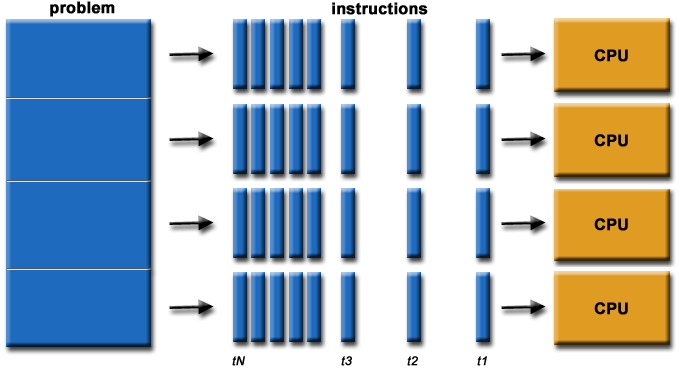
\includegraphics[width=0.8\textwidth]
		{pics/parallelProblem.png}
	\caption{Contoh masalah yang dikerjakan secara paralel}
	\label{fig:exmasalahparalel}
\end{figure}
\vspace{-0.8cm}
\begin{center}
{\small Sumber gambar: \citep{net.oxford}}
\end{center}

%-----------------------------------------------------------------------------%
\subsection{Klasifikasi X}
%-----------------------------------------------------------------------------%
Figure dalam enum dan dua sitasi sekaligus \citep{book.buyya,book.sterling-jones} :  
\begin{enumerate}
\item \bi{Bold Italic} \\
Penjelasan....... Untuk gambarannya dapat dilihat di Gambar \ref{fig:neumann}.

\begin{figure}
	\centering
	\includegraphics[height=0.65\textwidth,width=0.6\textwidth]
		{pics/neumann.pdf}
	\caption{Arsitektur klasik \f{von Neumann}}
	\label{fig:neumann}
\end{figure}
\vspace{-1.2cm}
\begin{center}
{\small Sumber gambar terinspirasi dari: \citep{buku.pressman}}
\end{center} 

\item \bi{Sesuatu banget} \\
Penjelasan.......
\end{enumerate}
\paragraph{}
%-----------------------------------------------------------------------------%
\section{\f{Section in Eng}}
%-----------------------------------------------------------------------------%
Hal pertama yang mungkin ditanyakan adalah bagaimana membuat huruf tercetak tebal, miring, atau memiliki garis bawah. 
Pada Texmaker, Anda bisa melakukan hal ini seperti halnya saat mengubah dokumen dengan LO Writer. 
Namun jika tetap masih tertarik dengan cara lain, ini dia: 

\begin{itemize}
	\item \bo{Bold} \\
		Gunakan perintah \bslash textbf$\lbrace\rbrace$ atau 
		\bslash bo$\lbrace\rbrace$. 
	\item \f{Italic} \\
		Gunakan perintah \bslash textit$\lbrace\rbrace$ atau 
		\bslash f$\lbrace\rbrace$. 
	\item \underline{Underline} \\
		Gunakan perintah \bslash underline$\lbrace\rbrace$.
	\item $\overline{Overline}$ \\
		Gunakan perintah \bslash overline. 
	\item $^{superscript}$ \\
		Gunakan perintah \bslash $\lbrace\rbrace$. 
	\item $_{subscript}$ \\
		Gunakan perintah \bslash \_$\lbrace\rbrace$. 
\end{itemize}

Perintah \bslash f dan \bslash bo hanya dapat digunakan jika package 
uithesis digunakan. 
%-----------------------------------------------------------------------------%
\subsection{Pengertian \f{Section in Eng}}
%-----------------------------------------------------------------------------%

%-----------------------------------------------------------------------------%
\subsection{Next Subsection \f{Section in Eng}}
%-----------------------------------------------------------------------------%

%-----------------------------------------------------------------------------%
\section{\f{Keatas lagi}}
%-----------------------------------------------------------------------------%
Contoh cite yang ga ada \cite{gaib}. Cite author \citeauthor{article.rebecca},cite tahun \citeyear{article.treese}, cite mention \cite{adin.experiment}, dan cite di akhir kalimat \citep{techreport.nist}.
%-----------------------------------------------------------------------------%
\subsection{\f{Masuk lagi}}
%-----------------------------------------------------------------------------%
Footnote example nih : MPICH \footnote{\url{http://www.mpich.org/}}, LAM/MPI \footnote{\url{http://www.lam-mpi.org/}}, dan OpenMPI \footnote{\url{www.open-mpi.org}} \citep{article.mcguire}. MPI-3 sedang dalam tahap perencanaan \footnote{\url{http://meetings.mpi-forum.org/MPI_3.0_main_page.php}}. Fungsi-fungsi tersebut berada di tabel \ref{tab:mpifund}. (Contoh tabel).

\begin{table}
	\centering
	\caption{Fungsi fundamental MPI}
	\label{tab:mpifund}
	\begin{tabular}{|c|c|c|}
	\hline
	\rowcolor{headertbl}	
	\hline No. & Nama Fungsi & Penjelasan \\ 
	\hline 1 & MPI\_Init & Memulai kode MPI \\ 
	\hline 2 & MPI\_Finalize & Mengakhiri kode MPI \\ 
	\hline 3 & MPI\_Comm\_size & Menentukan jumlah proses \\ 
	\hline 4 & MPI\_Comm\_rank & Menentukan label proses \\ 
	\hline 5 & MPI\_Send & Mengirim pesan \\ 
	\hline 6 & MPI\_Recv & Menerima pesan \\ 
	\hline
	\end{tabular}
\end{table}
\begin{center}
{\small Sumber tabel: taro sitasi disini, if i were u}
\end{center}
%-----------------------------------------------------------------------------%
\chapter{\babTiga}
%-----------------------------------------------------------------------------%
Bagian ini akan menjelaskan mengenai metodologi penelitian yang digunakan dalam penelitian ini. Metodologi tersebut meliputi pendekatan penelitian, populasi dan sampel penelitian, tahapan penelitian, model penelitian, instrumen penelitian, metode pengumpulan data, hipotesis awal dan teknik analisis data.
%-----------------------------------------------------------------------------%
\section{Pendekatan Penelitian}
%-----------------------------------------------------------------------------%
Penelitian dilakukan dengan menggunakan pendekatan secara kuantitatif dan kualitatif. Pendekatan kuantitatif adalah suatu teknik pengumpulan data melalui media-media yang telah ditentukan dan menghasilkan data statistik \citep{buku.creswell}. \citeauthor{buku.creswell} menjelaskan bahwa terdapat dua strategi yang dapat dilakukan pada pendekatan kuantitatif, yaitu eksperimen dan survei. Dalam penelitian ini penulis melakukan eksperimen dengan pelaksanaan \ust. Selanjutnya pendekatan kualitatif adalah suatu teknik pengumpulan data dan analisis terhadap data-data yang sifatnya tidak numerik. Pada penelitian ini diperoleh data yang bersifat kuantitatif dimana diperoleh dari tanggapan responden terhadap \f{website} melalui kuesioner dengan skala likert serta data kualitatif yang diperoleh dari preferensi, rekomendasi dan saran responden terhadap \f{website}.
%-----------------------------------------------------------------------------%
\section{Populasi dan Sampel}
%-----------------------------------------------------------------------------%
Populasi yang digunakan dalam penelitian ini adalah mahasiswa dengan jurusan Administrasi di lingkungan Universitas Indonesia, konsultan pajak dan pekerja di bidang pajak. Populasi ini dipilih berdasarkan pada pemahaman dan kebutuhan pengguna terhadap \f{website} direktorat jenderal pajak. Adapun sampel pada penelitian ini adalah 36 orang terpilih dari populasi dengan komposisi 11 orang mahasiswa serta 25 orang konsultan dan pekerja di bidang pajak. Pemilihan sampel dalam penelitian ini menggunakan metode \textit{purposive sampling}, dimana penulis mencari responden yang sesuai dengan kriteria pada populasi. Adapun kriteria dalam penelitian ini adalah mahasiswa dan pekerja di bidang pajak yang sudah pernah membuka \f{website} direktorat jenderal pajak Indonesia.
%-----------------------------------------------------------------------------%
\section{Tahapan Penelitian}
%-----------------------------------------------------------------------------%
Tahapan yang dilakukan pada penelitian ini adalah perumusan masalah, studi literatur, penyusunan rancangan penelitian, pengumpulan data (eksperimen), analisis data, perancangan \f{prototype}, evaluasi \f{prototype} dan penarikan kesimpulan.
%-----------------------------------------------------------------------------%
\subsection{Perumusan Masalah}
Pada tahap ini dilakukan perumusan masalah yang akan diangkat dalam penelitian. Permasalahan yang diangkat adalah kemudahan, kenyamanan dan fungsionalitas penggunaan sistem \f{e-government} berbasis \f{website} melalui tampilan antarmuka dan \f{user experience}. Kenyamanan, kemudahan dan fungsionalitas ini ditujukan untuk meningkatkan produktifitas pengguna dalam menggunakan sistem serta pelayanan dari sistem yang semakin baik.
%-----------------------------------------------------------------------------%
\subsection{Studi Literatur}
Pada tahap ini dilakukukan studi literatur dengan cara pencarian definisi dan teori penunjang. Hasil pencarian digunakan untuk pembuatan model penelitian yang dilakukan. Proses studi literatur yang dilakukan meliputi teori \f{e-government}, pengujian \f{e-government}, \ust, \f{website} direktorat jenderal pajak serta teori lainnya yang berkaitan dengan permasalahan pada penelitian.
%-----------------------------------------------------------------------------%
\subsection{Penyusunan Rancangan Penelitian}
Pada tahap ini dilakukan penyusunan rancangan penelitian. Rancangan penelitian terdiri dari beberapa komponen dengan menjalankan \ust. Komponen-komponen tersebut adalah sebagai berikut:
%-----------------------------------------------------------------------------%
\subsubsection{Mengembangkan \f{Test Plan}}
\f{Test plan} dalam \ust \space merupakan tahapan yang penting dimana menurut \citet{buku.rubin} \f{test plan} berfungsi sebagai peta pengujian, kendaraan komunikasi yang utama,  menyiratkan kebutuhan dasar, dan juga menyediakan titik fokus pengujian menjadi sebuah pencapaian. \citeauthor{buku.rubin} menjabarkan \f{test plan} menjadi beberapa bagian seperti berikut:
\begin{enumerate}[label=\alph*.]
	\item Menentukan maksud, capaian dan tujuan dari \f{test}\\
	Pada tahap ini ditinjau kembali maksud dan tujuan dari \ust \space serta meninjau ulang capaian yang ingin diraih dari hasil pengujian. Bagian ini akan dijelaskan pada subbab 3.3.1 dan subbab 3.3.6.
	\item Menentukan target pengguna\\
	Tahap ini menjelaskan mengenai target pengguna yang akan menjadi responden dalam proses \ust. Pengguna dalam penelitian ini merupakan refleksi dari pengguna sistem. Pengguna yang dipilih menjadi responden \ust \space ini telah dijelaskan pada subbab 3.2.
	\item Menentukan dan menetapkan metode \f{test design}\\
	Pada tahap ini dilakukan penetapan dan penentuan \f{test} yang akan dilakukan. Proses penentuan dan penetapan meliputi prosedur \f{testing} dan prosedur pengumpulan data. Berikut merupakan prosedur yang dilakukan dalam penelitian ini:
	\begin{itemize}
		\item Proses pengumpulan data dilakukan pada tanggal 18 Mei 2015 sampai dengan 1 Juni 2015.
		\item \f{Usability testing} dilakukan dengan menggunakan komputer pribadi milik penulis ataupun pengguna yang sudah disiapkan sebelumnya. 
		\item Penulis selaku penguji membebaskan kepada responden untuk melakukan eksplorasi terhadap sistem \f{website} selama pengerjaan tugas yang telah diberikan.
		\item Penulis selaku penguji hanya bertindak mengamati dan menjadi moderator selama pengujian.
	\end{itemize} 
	\item Merancang dan Menentukan daftar tugas dan kuesioner pengujian\\
	Pada bagian ini penulis melakukan perancangan terkait tugas dan kuesioner yang akan kepada responden dalam \ust. Deskripsi lebih lanjut mengenai tahap ini akan dijelaskan pada subbab 3.3.3.2.
	\item Menyiapkan lingkungan penelitian dan perlengkapan pengujian\\
	Pada tahap ini ditentukan persiapan untuk melaksanakan penelitian (pengumpulan data). Lingkungan penelitian yang disiapkan penulis adalah lokasi yang kondusif untuk melakukan moderasi, seperti tempat yang memiliki ruang gerak cukup luas. Perlengkapan yang disiapkan penulis dalam melaksanakan \ust \space adalah sebagai berikut:
	\begin{itemize}
		\item 1 buah PC yang akan digunakan responden dalam \ust,
		\item Skenario pengujian,
		\item Kuesioner dan
		\item \f{Stopwatch}
	\end{itemize}
\end{enumerate}
%-----------------------------------------------------------------------------%
\subsubsection{Perancangan tugas dan kuesioner}
Dalam perancangan tugas penulis memakai acuan berdasar fitur yang dimiliki oleh \f{website} direktorat jenderal pajak baik Indonesia maupun India. Fitur yang memiliki kesamaan kemudian dikelompokkan menjadi poin tugas yang akan dilakukan oleh responden. Tugas-tugas disusun berdasar dengan materi komponen pengujian yang sudah dijelaskan pada subbab \ref{subsec:nush} dan \ref{subsec:gquality}.
Berikut merupakan daftar tugas yang diberikan pada responden:
\begin{enumerate}
	\item Melakukan pengamatan halaman utama sistem \f{website},
	\item Pengamatan Desain halaman artikel dan fitur arsip artikel,
	\item Melakukan pengunduhan berkas dari arsip unduhan,
	\item Eksplorasi halaman bantuan dan dokumentasi,
	\item Eksplorasi halaman terkait pengumuman,
	\item Eksplorasi halaman keterbukaan informasi terkait informasi lelang,
	\item Menggunakan sistem pencarian \f{website} berdasar kata kunci,
	\item Pencarian kontak informasi,
	\item \f{Login} aplikasi \f{e-filling} dan melakukan kegiatan pengamatan beserta eksplorasi fitur yang ada, seperti pengelolaan item form yang ada dan \f{logout} sistem, serta
	\item Uji coba pranala yang berkaitan dengan sistem.
\end{enumerate}
Penyusunan tugas yang diberikan terhadap responden telah diatur sedemikian rupa agar mereprentasikan tujuan dalam penelitian ini. Tugas tersebut diproyeksikan kedalam skenario pengujian.
\newline\\
Untuk melaksanakan pengujian terhadap \f{website} \f{e=government}, dirancang sebuah kuesioner yang dapat mengumpulkan data penilaian \f{website}. Kuesioner ini disusun berdasarkan komponen-komponen yang dijabarkan pada subbab \ref{subsec:nush} dan \ref{subsec:gquality}. Adapun rancangan kuesioner \ust \space terdiri dari beberapa bagian sebagai berikut:
\begin{enumerate}
	\item Biodata Responden\\
	Pada bagian ini kuesioner berisikan mengenai biodata dan informasi terkait responden yang dibutuhkan untuk tahap analisis demografi.
	\item Komponen \f{Usability}\\
	Bagian komponen \f{usability} berfungsi sebagai alat ukur untuk mendapatkan nilai \f{usability heuristic}. Berikut merupakan tabel pertanyaan dari kuesioner komponen \f{usability heuristic} yang diberikan kepada responden:
\begin{center}
	\begin{longtable}{|p{11.2cm}|}
		\caption{Tabel Kuesioner Komponen \f{Usability Heuristic}}	\\	
			\hline
			\multicolumn{1}{|c|}{{\bf Pertanyaan}}\\ 
			\hline
			{\bf Visibility of system status}                                                                           \\
			Feedback yang diberikan sistem membuat saya mengetahui apa yang sedang saya lakukan.                        \\ \hline
			{\bf Match between system and real world}                                                                   \\
			Istilah yang digunakan sudah jelas deskriptif dan familiar bagi saya.                                       \\
			Informasi yang diberikan mudah dimengerti.                                                                  \\ \hline
			{\bf User control}                                                                                          \\
			Saya dapat melakukan pembatalan terhadap suatu task.                                                        \\ \hline
			{\bf Consistency and standards}                                                                             \\
			Istilah jenis font dan design yang digunakan konsisten.                                                     \\ \hline
			{\bf Error prevention}                                                                                      \\
			Saya mengerti keterangan yang diberikan pada sistem.                                                        \\
			Keterangan pada sistem membuat saya tidak melakukan kesalahan.                                              \\ \hline
			{\bf Recognition rather than recall}                                                                        \\
			Letak menu dan icon yang digunakan membantu saya untuk mengetahui tujuan dan fungsinya.                     \\
			Saya dapat mengingat dengan mudah bagaimana cara menggunakan sistem.                                        \\ \hline
			{\bf Flexibility and efficiency of use}                                                                     \\
			Saya mengerti tujuan dari sistem ini secara keseluruhan.                                                    \\
			Saya mengerti tujuan dari menu yang digunakan.                                                              \\
			Saya dapat menggunakan sistem dengan mudah.                                                                 \\ \hline
			{\bf Aesthetic and Minimalist Design}                                                                       \\
			Setelah menggunakan sistem saya menilai sistem ini menarik (dari segi tampilan dan tata letak).             \\
			Saya tidak keberatan untuk berlama-lama menggunakan sistem ini.                                             \\ \hline
			{\bf Help user recognize diagnose and recover from errors}                                                  \\
			Ketika saya melakukan kesalahan sistem memberikan petunjuk sehingga saya dapat memperbaikinya dengan mudah. \\ \hline
			{\bf Help and documentation}                                                                                \\
			Informasi tambahan (fitur help/FAQ) membuat saya mengerti ketika mengalami kesulitan.                       \\ \hline
	\end{longtable}
\end{center}
	\item Komponen Kepuasan Pengguna\\
	Komponen ini menjelaskan mengenai kepuasan pengguna terhadap \f{website} yang dievaluasi. Berikut merupakan tabel pertanyaan kepuasan pengguna yang terdapat dalam kuesioner:
	\begin{table}
		\centering
		\caption{Tabel Kuesioner Komponen Kepuasan Pengguna}
		\begin{tabular}{|p{11.2cm}|}
			\hline
			\multicolumn{1}{|c|}{{\bf Pertanyaan}}						\\ \hline
			Saya merasa mudah dan nyaman untuk menggunakan sistem ini.	\\ \hline
			Saya membutuhkan sistem ini untuk membantu pekerjaan saya.	\\ \hline
			Saya akan merekomendasikan sistem ini kepada orang lain.	\\ \hline
		\end{tabular}
	\end{table}
	\item Komponen \f{g-Quality}\\
	Komponen ini merupakan komponen untuk mengevaluasi nilai \f{website} \f{e-government} berdasarkan kategori yang sudah dijelaskan pada subbab \ref{subsec:gquality}. Berikut merupakan tabel pertanyaan komponen \f{g-quality} yang terdapat pada kuesioner:
	\begin{center}
	\begin{longtable}{|p{11.2cm}|}
		\caption{Kuesioner Komponen Kepuasan Pengguna} \\
		\hline
			\multicolumn{1}{|c|}{{\bf Pertanyaan}}										\\ \hline
			{\bf Accessibility}															\\
			Sistem dapat digunakan dan dioperasikan oleh semua kalangan.               	\\ \hline
			{\bf Interoperability}                                                      \\
			Dapat melakukan pertukaran data dan informasi dengan sistem E-Gov lainnya.  \\ \hline
			{\bf Security and Privacy}                                                  \\
			Sistem dapat mencegah terjadinya kebocoran data yang dimiliki pengguna.     \\ \hline
			{\bf Information Truth and Precision}                                       \\
			Saya merasa sistem menyampaikan informasi yang benar, akurat dan terkini.   \\ \hline
			{\bf Service Agility}                                                       \\
			Saya merasa penggunaan sistem cepat dan mudah diakses.                      \\ \hline
			{\bf Transparency}                                                          \\
			Saya merasa informasi yang disampaikan sistem sudah transparan.				\\ \hline
	\end{longtable}
\end{center}
\end{enumerate}
%-----------------------------------------------------------------------------%
\subsubsection{Menentukan tipe data}
Tipe data yang digunakan dalam penelitian ini adalah sebagai berikut:
\begin{enumerate}
	\item Kuantitatif\\
	Tipe data kuantitatif terdiri dari waktu yang dibutuhkan responden dalam pengerjaan tugas dan juga penilaian yang diberikan responden terhadap komponen pengujian dalam kuesioner.
	\item Kualitatif\\
	Tipe data kualitatif pada penelitian ini terdiri dari penilaian tertulis, rekomendasi dan saran dari responden terhadap \f{website} dan \f{prototype}.
\end{enumerate}
%-----------------------------------------------------------------------------%
\subsubsection{Persiapan pelaksanaan \ust}
Sebelum melaksanakan \ust, penulis selaku penguji melakukan beberapa aktifitas seperti \f{checklist} dalam persiapan pengujian seperti yang disampaikan \citet{buku.rubin}. Berikut merupakan daftar \f{checklist} yang dilakukan penulis dalam persiapan pelaksanaan pengujian:
\begin{enumerate}
	\item \f{Checklist 1: Test Preparation}\\
	Sebelum masuk ke masa pengujian, penulis melakukan \f{selftest} dan \f{pilot test} terlebih dahulu dengan tujuan memberikan gambaran pada saat pengujian yang akan dilaksanakan nanti. Berikut merupakan tahapan yang dilakukan pada \f{test preparation} ini:
	\begin{itemize}
		\item Melakukan \f{self test} untuk menyesuaikan skenario pengujian dengan sistem yang akan diujikan.
		\item Melaksanakan \f{pilot test} yang dilakukan oleh satu orang sukarelawan untuk menguji skenario dan pelaksanaan \ust \space sebagai simulasi. 
		\item Melakukan uji keterbacaan kuesioner dan skenario bersama 5 orang sukarelawan secara acak dengan maksud mendapat \f{feedback} untuk dilakukan perbaikan nantinya.
		\item Revisi kuesioner dan skenario berdasarkan pengujian pada tahap sebelumnya.
	\end{itemize}
	\item \f{Checklist 2: Pre-test}\\
	Penulis melakukan persiapan sebelum melaksanakan pengujian terhadap responden dengan mempersiapkan perlengkapan seperti PC siap pakai, jaringan yang sudah terkoneksi dan membagikan skenario \f{testing} yang telah disiapkan.
	\item \f{Checklist 3: Test Monitor Activities}\\
	Penulis melakukan monitoring dan moderasi pada saat pelaksanaan \ust. Aktifitas monitoring ini ditujukan untuk memastikan data sudah terisi dengan benar serta melakukan rekap data terkait kesalahan, waktu dan catatan selama \ust \space berlangsung.
\end{enumerate}
%-----------------------------------------------------------------------------%
\subsection{Pelaksanaan Penelitian}
Pada tahap ini penulis melakukan \ust \space terhadap \f{website} \f{e-government} dengan mengikuti aturan yang dijelaskan oleh \citet{buku.rubin} dan \citet{buku.dumas} sebagai berikut:
\begin{enumerate}
	\item Perkenalan\\
	Pada bagian ini penulis melakukan perkenalan terhadap responden dan menjelaskan mengenai latar belakang penelitian, skenario \f{testing} dan pengisian kuesioner.
	\item \f{Pre-test briefing}\\
	Sebelum memasuji sesi pengujian, penulis melakukan \f{briefing} terhadap responden yang menjelaskan mengenai kegiatan yang akan dilakukan dan mempersilahkan responden untuk melakukan eksplorasi terhadap \f{website} yang diujikan.
	\item Sesi \f{test}\\
	Pada saat sesi ini responden menjalankan tugas sesuai dengan skenario yang telah disiapkan sebelumnya. Penulis bertugas menjadi moderator dan fasilitator pada saat \f{test} berjalan.
	\item \f{Post-test debriefing}\\
	Setelah sesi pengujian selesai dilakukan oleh responden, penulis menjelaskan kembali terkait cara pengisian kuesioner dan memandu responden dalam melakukan pengisian kuesioner yang telah diberikan.
\end{enumerate}
%-----------------------------------------------------------------------------%
\subsection{Analisis Data dan \f{Requirement Gathering}}
Pada tahap ini dilakukan analisis data dari hasil \ust \space dengan responden  dengan metode yang dijelaskan pada subbab 3.5 dan mengumpulkan \f{requirement} dari hasil analisis rekomendasi responden untuk mengembangkan \f{clickable-prototype}. 
%-----------------------------------------------------------------------------%
\subsection{Perancangan \f{Prototype}}
Pada tahap ini penulis melakukan perancangan \f{prototype} yang dibuat berdasarkan hasil \ust \space dengan responden. Penulis mengembangkan prototype dengan aplikasi berbasis web \textbf{invisionapp} yang sudah dijelaskan pada subbab \ref{subsec:invisionapp}. 
%-----------------------------------------------------------------------------%
\section{Metode Pengumpulan Data}
%-----------------------------------------------------------------------------%
Pada bagian ini dijelaskan mengenai metode pengumpulan data beserta jenis dan sumber data yang digunakan pada penelitian.  
%-----------------------------------------------------------------------------%
\subsection{Jenis dan Sumber Data}
Penelitian ini menggunakan sumber data primer yang diperoleh langsung dari orang pertama, yakni dari responden secara langsung. Penelitian ini menggunakan dua jenis data, yaitu data subjektif dan data objektif.
\begin{enumerate}
	\item Data Subjektif\\
	Data subjektif dalam penelitian ini diperoleh dari kuesioner yang menggunakan skala likert serta rekomendasi dan saran dari responden. Skala likert digunakan sebagai penilaian subjektif responden terhadap \f{website} \f{e-government} yang diujikan dan rekomendasi sebagai bagian dari masukkan responden untuk peningkatan fitur atau aspek tertentu dari \f{website} yang diujikan. 
	\item Data Objektif\\
	Data objektif dalam penelitian ini diperoleh dari hasil pengukuran data kuantitatif yang diakukan oleh penulis sebagai moderetor dan fasilitator dalam pelaksanaan \ust. Data objektif meliputi waktu pengerjaan tugas selama pengujian dan jumlah kesalahan tugas yang dilakukan oleh responden.
\end{enumerate}
%-----------------------------------------------------------------------------%
\subsection{Teknik Pengumpulan Data}
Penulis melakukan beberapa cara untuk melakukan pengumpulan data seperti berikut:
\begin{enumerate}
	\item Observasi\\
	Metode ini digunakan pada saat melakukan penelitian dengan mengumpulkan data secara langsung melalui pengamatan terhadap responden pada saat \ust \space berlangsung. Observasi yang dilakukan adalah melihat, mengukur waktu, menghitung serta mencatat kejadian yang ada pada saat \ust. Pengukuran waktu dilakukan dengan menghitung waktu kinerja responden dalam pengerjaan tugas secara keseluruhan, sedangkan penghitungan dilakukan dengan mencatat jumlah kesalahan dan masalah yang dialami oleh responden.
	\item Kuesioner\\
	Kuesioner dideskripsikan oleh \citet{buku.riduwan} sebagai daftar pertanyaan yang diberikan kepada orang lain yang bersedia memberikan respons (responden) sesuai dengan permintaan pengguna. \citeauthor{buku.riduwan} menjelaskan tujuan dari kuesioner adalah untuk mencari informasi yang lengkap mengenai suatu masalah dan reponden tidak merasa khawatir bila memberikan jawaban yang diberikan tidak sesuai dengan kenyataan dalam pengisian daftar pertanyaan.
	Adapun jenis pertanyaan yang disajikan pada kuesioner yaitu \citep{buku.riduwan}:
	\begin{enumerate}
		\item Pertanyaan terbuka\\
		Kuesioner dengan jenis pertanyaan terbuka (tidak memiliki struktur) adalah kuesioner yang disajikan dalam bentuk sederhana sehingga responden dapat memberikan isian sesuai dengan kehendak dan keadaannya. Dalam penelitian ini terdapat bagian dari kuesioner yang memiliki pertanyaan terbuka seperti pada bagian rekomendasi dan preferensi responden.
		\item Pertanyaan tertutup\\
		Pertanyaan tertutup dijelaskan sebagai kuesioner yang disajikan dalam bentuk sedemikian rupa sehingga responden diminta untuk memilih satu jawaban yang sesuai dengan karakteristik dirinya dengan cara menandai pilihan (dapat berupa skala atau pilihan ganda) pada pertanyaan. Pada penelitian ini digunakan skala likert sebagai pilihan yang terdapat pada kuesioner. Skala likert adalah skala yang digunakan untuk mengukur sikap, pendapat dan persepsi seseorang atau sekelompok tentang kejadian atau gejala sosial \citep{buku.riduwan}. Skala likert yang digunakan penulis adalah sebagai berikut:
		\begin{table}
			\centering
			\caption{Skala Likert pada Kuesioner}
			\label{tab:tab2}
			\begin{tabular}{|c|l|}
				\hline
				{\bf Skala} & \multicolumn{1}{c|}{{\bf Keterangan}} \\ \hline
				1           & Sangat tidak setuju                   \\ \hline
				{\it 2}     & Tidak setuju                          \\ \hline
				3           & Agak tidak setuju                     \\ \hline
				{\it 4}     & Netral                                \\ \hline
				5           & Agak setuju                           \\ \hline
				6           & Setuju                                \\ \hline
				7           & Sangat setuju                         \\ \hline                      
			\end{tabular}
		\end{table}
	\end{enumerate}
\end{enumerate}
%-----------------------------------------------------------------------------%
\section{Metode Analisis Data}
Metode analisis data yang digunakan pada penelitian ini adalah metode statistik \f{paired samples t-test} yang melakukan uji rata-rata pada dua buah kelompok data yang saling berhubungan. Data yang diolah dalam metode ini adalah data yang bersifat parametrik dengan bentuk interval dan terdistribusi secara normal. Diperlukan uji normalitas untuk melihat apakah data terdistribusi secara normal. Dikarenakan data dalam penelitian ini bersifat ordinal dengan skala kategori lebih dari 4, maka penulis tidak perlu melakukan konversi nilai ordinal menjadi interval karena menurut \citet{ho.newsom} data ordinal dengan skala kategori lebih dari 5 dapat langsung dihitung dan dianalisa dengan metode parametrik.
%-----------------------------------------------------------------------------%
\subsection{Uji Normalitas}
Uji normalitas bertujuan untuk menguji apakah data terdistribusi normal. \citet{ppt.schwab} mengatakan bahwa terdapat dua cara untuk mengevaluasi normalitas. Pertama adalah dengan metode statistikal, lalu kedua menggunakan pengamatan grafis. Metode grafis menggunakan histogram dan plot normalitas dalam pengamatannya. Gambar \ref{fig:histogramnormal} menunjukan histogram yang terdistribusi normal. Sedangkan metode statistikal melakukan diagnosa hipotesis tes untuk normalitas dan variabelnya mendekati normal jika \f{skewnes} dan \f{kurtosis} memiliki nilai antara -2.0 dan 2.0, gambar \ref{fig:grafiknormal} menunjukan grafik dataset yang terdistribusi normal. Menurut \citet{buku.sugiyono}, salah satu uji normalitas data adalah dengan metode chi kuadrat ($x^2$) dimana pengujian hipotesis dilakukan dengan cara membandingkan kurva normal yang terbentuk dari data yang telah terkumpul (B) dengan kurva normal standar (A). Bila B tidak berbeda secara signifikan dengan A, maka B merupakan data yang berdistribusi normal. Cara lain untuk melakukan uji normalitas adalah dengan metode deskriptif, dimana metode ini menghitung \f{skewness} dan nilai \f{kurtosis}, setelah itu dilakukan transformasi kedua nilai tersebut dengan \f{z-score}. 
\newline\\
Suatu besaran statistik yang menunjukan kemiringan data disebut \f{skewness}, data \f{skewnes} memiliki kecenderungan berada di tengah atau miring di satu sisi saja. Sedangkan \f{kurtosis} merupakan keruncingan data \citep{article.setiawan}. Rasio \f{skewnes} dapat diperoleh dari rumus:
\begin{equation}
\centering
 Z_{skewnes} = \cfrac{s-0}{SE_{skewness}} 
\end{equation}
Dengan nilai \f{skewness} adalah \f{s} dan SE nilai \f{standard error}. Data terdistribusi normal jika berada pada rentang -1.0 sampai 1.0. Sedangkan nilai rasio kurtosis dapat diperoleh dengan persamaan berikut:
\begin{equation}
\centering
Z_{kurtosis} = \cfrac{s-0}{SE_{skewness}} 
\end{equation}

\begin{figure}[ht]
	\centering
	\begin{minipage}[b]{0.45\linewidth}
		\centering
		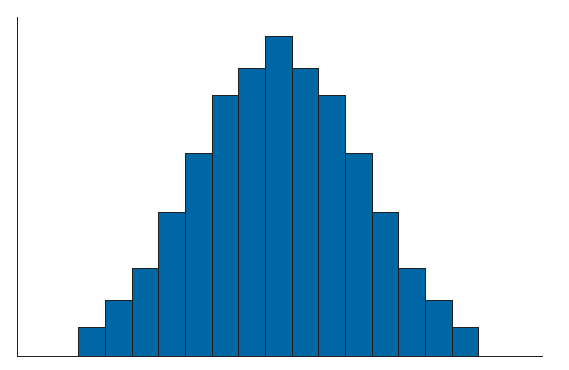
\includegraphics[width=\textwidth]{pics/histogram-normal.png}
		\caption{Histogram \f{Normal Distribution Dataset}}
		\label{fig:histogramnormal}
	\end{minipage}
	\hspace{0.5cm}
	\begin{minipage}[b]{0.45\linewidth}
		\centering
		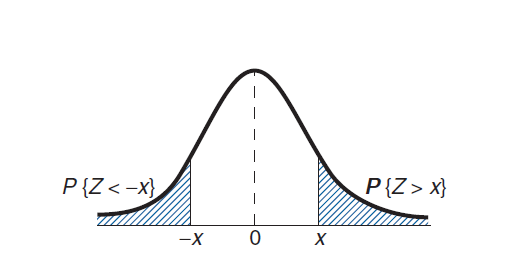
\includegraphics[width=\textwidth]{pics/normal-distribution.png}
		\caption{Grafik \f{Normal Distribution Dataset}}
		\label{fig:grafiknormal}
	\end{minipage}
\end{figure}
\begin{center}
	{\small Sumber gambar: \citep{buku.ross}}
\end{center}
Bila data tidak terdistribusi secara normal, maka dapat dilakukan uji normalisasi dengan mentransformasi data. Transformasi data dapat dilakukan dengan aplikasi SPSS pada menu "Compute Variable". \citet{buku.field} menjelaskan bahwa penghitungan uji normalitas pada SPSS dapat dilakukan dengan cara seperti berikut:
\begin{enumerate}
	\item \f{Log Transformation}\\
	Bila data bersifat \f{positive skew} maka digunakan metode ini untuk memperbaiki data yang memiliki \f{unequal variances}. Bila data memiliki nilai 0 atau bernilai negatif, maka dilakukan $log(X_{1}+1)$ untuk membuat data tetap positif.
	\item \f{Square Root Transformation}\\
	Metode ini digunakan untuk mengurai \f{positive skew} dengan mengambil akar kuadrat dari masing-masing data. Metode ini memiliki kekurangan ketika mengurai data yang memiliki nilai negatif, hal ini disebabkan nilai negatif tidak memiliki nilai akar kuadrat.
	\item \f{Reciptocal Transformation}\\
	Metode ini digugnakan untuk memperbaiki data yang bersifat \f{negative skew} dengan melakukan pembagian angka 1 oleh masing-masing nilai data.
\end{enumerate}
Setiap metode transformasi diatas dapat digunakan untuk memperbaiki data yang \f{negatif skew} dengan melakukan \f{reverse score}.
%-----------------------------------------------------------------------------%
\subsection{\f{Paired Samples t-Test}}
Metode ini merupakan salah satu metode uji hipotesis komparatif untuk dua buah data yang saling berhubungan. \citet{article.shier} menyebutkan bahwa perbandingan dua populasi dilakukan bilamana sampel observasi dapat dibandingkan dengan observasi lainnya. \citeauthor{article.shier} mengeluarkan prosedur manual untuk melakukan t-Test sebagai berikut:
\begin{enumerate}
	\item Hitung perbedaan ($d_{i} = y_{i}-x_{i}$) antara dua populasi untuk menghilangkan perbedaan positif dan negatif.
	\item Hitung \f{mean} perbedaan $\overline{d}$.
	\item Hitung standar deviasi dari perbedaan $S_{d}$, lalu gunakan nilai tersebut untuk menghitung standar error dari \f{mean} perbedaan, $SE(\overline{d}) = \cfrac{S_{d}}{\sqrt{n}}$.
	\item Hitung t-statistic, dengan $T = \cfrac{\overline{d}}{SE(\overline{d})}$. Dengan dilandasi \f{null hypothesis}, maka statistik ini mengikuti \f{t-distribution} dengan derajat kebebasan n-1.
	\item Gunakan tabel \f{t-distribution} untuk membandingkan nilai T terhadap distribusi $t_{n-1}$ dan akan memberikan nilai \f{p-value} dari \f{t-test} yang dibandingkan.
\end{enumerate}
Selain langkah diatas, dapat juga digunakan aplikasi SPSS untuk menghitung nilai perbedaan dengan langkah seperti berikut:
\begin{enumerate}
	\item Memeriksa syarat \f{paired sample t-test} dimana sebaran data harus terdistribusi normal. Bila data tidak terdistribusi normal maka lakukan transformasi data.
	\item Lakukan penghitungan \f{paired sample t-test} terhadap data yang sudah di transformasi dengan sebaran data terdistribusi normal.
	\item Jika variabel hasil transformasi masih belum memiliki data yang terdistribusi normal, maka dilakukan metode \f{Wilcoxon signed-rank test}.
\end{enumerate}
\f{Paired sample t-test} dapat dilakukan pada aplikasi SPSS dengan langkah pemilihan menu \textbf{Analyze $\rightarrow$ Compare Means $\rightarrow$ Paired Samples t-test}. Bila nilai \f{significancy} data kurang dari 0.05 (p < 0.05) maka terdapat perbedaan signifikan antara kedua \f{mean} kelompok data dan sebaliknya.
%-----------------------------------------------------------------------------%
%-----------------------------------------------------------------------------%
\chapter{\babEmpat}
%-----------------------------------------------------------------------------%
Pada bagian ini dijelaskan mengenai data hasil penelitian dan analisis data yang dilakukan oleh penulis. Hasil penelitian meliputi data demografi responden dan hasil pengolahan data yang diperoleh dari survei yang telah dilaksanakan pada masing-masing variabel pengukuran, analisis teori serta pengolahan rekomendasi responden pada penelitian.
%-----------------------------------------------------------------------------%
\section{Demografi Responden}
Pada penelitian ini responden adalah target pengguna dari \f{website} Direktorat Jenderal Pajak (DJP). Responden berjumlah 36 orang yang merupakan orang yang bekerja di bidang pajak serta mahasiswa dengan jurusan administrasi perpajakan(fiskal). Berikut merupakan grafik demografi dari responden penelitian.
\begin{figure}
	\centering
	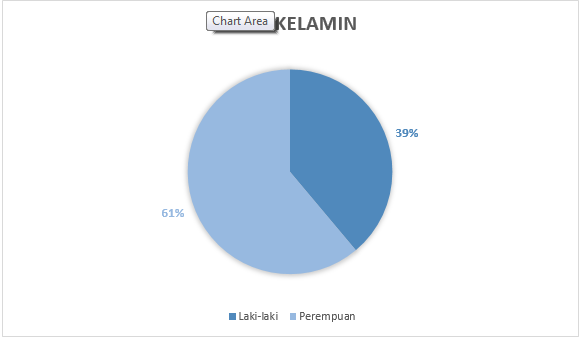
\includegraphics[width=0.9\textwidth,height=0.52\textwidth]
	{pics/jenisKelamin.PNG}
	\caption{Persentase jenis kelamin responden}
	\label{fig:jeniskelamin}
\end{figure}
\noindent
Gambar \ref{fig:jeniskelamin} menampilkan persentase data berdasarkan jenis kelamin responden. Diketahui dari gambar tersebut terdapat 14 orang laki-laki (39\%) dan 22 orang perempuan (61\%) yang menjadi responden. Gambar \ref{fig:kerja} merepresentasikan profesi yang dimiliki oleh responden berdasarkan jenisnya. Dari gambar dapat dilihat terdapat 19 orang (53\%) yang berprofesi sebagai konsultan pajak, 6 orang (17\%) pada bidang pajak lainnya dan 11 orang (30\%) mahasiswa dari jurusan administrasi perpajakan (fiskal).
\begin{figure}
	\centering
	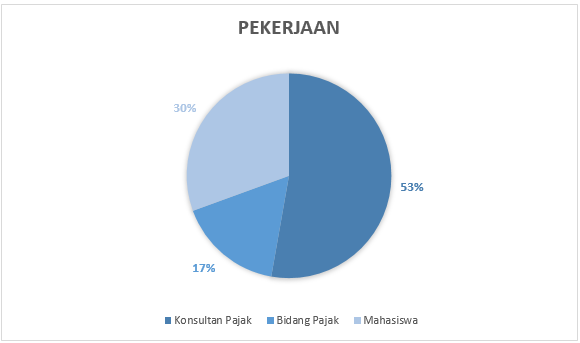
\includegraphics[width=0.9\textwidth,height=0.52\textwidth]
	{pics/pekerjaan.PNG}
	\caption{Persentase pekerjaan responden}
	\label{fig:kerja}
\end{figure}
\begin{figure}
	\centering
	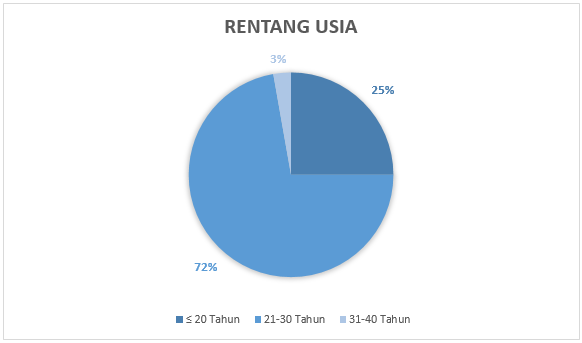
\includegraphics[width=0.9\textwidth,height=0.52\textwidth]
	{pics/rentangUsia.PNG}
	\caption{Persentase rentang usia responden}
	\label{fig:usia}
\end{figure}
\noindent
Gambar \ref{fig:usia} menggambarkan data persentase rentang usia responden penelitian. Diketahui dari gambar tersebut terdapat 1 orang (3\%) yang berusia pada rentang 31-40 tahun, 26 orang (72\%) yang berusia pada rentang 21-30 tahun serta 9 orang (25\%) responden yang berusia dibawah atau sama dengan 20 tahun.
\begin{figure}
	\centering
	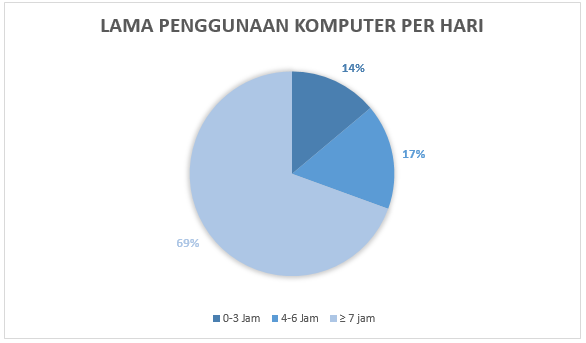
\includegraphics[width=0.9\textwidth,height=0.52\textwidth]
	{pics/lamakomputer.PNG}
	\caption{Persentase lama penggunaan komputer per hari responden}
	\label{fig:komp}
\end{figure}
\noindent
Gambar \ref{fig:komp} menunjukan persetase lama penggunaan komputer responden per hari. Sebanyak 5 orang (14\%) responden menggunakan komputer 0-3 Jam per hari, 6 orang (17\%) responden menggunakan komputer selama 4-6 jam per hari dan 25 oranng (69\%) responden menggunakan komputer selama lebih dari sama dengan 7 jam pada tiap harinya.
\begin{figure}
	\centering
	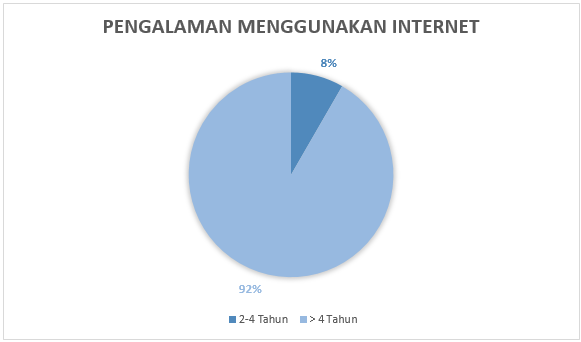
\includegraphics[width=0.9\textwidth,height=0.52\textwidth]
	{pics/pengalamanInternet.PNG}
	\caption{Persentase pengalaman responden menggunakan internet}
	\label{fig:lamainet}
\end{figure}
\noindent
Gambar \ref{fig:lamainet} menjelaskan mengenai persentasi pengalaman responden dalam menggunakan internet. Terdapat 3 orang (8\%) responden yang memiliki pengalaman menggunakan internet selama 2-4 tahun dn 33 orang (92\%) responden yang memiliki pengalaman menggunakan internet selama lebih dari 4 tahun.
\begin{figure}
	\centering
	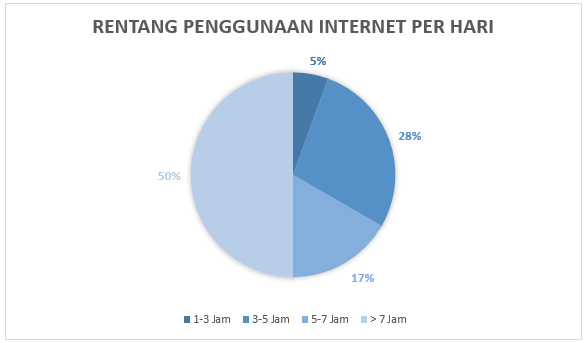
\includegraphics[width=0.9\textwidth,height=0.52\textwidth]
	{pics/pakeInternetperhari.PNG}
	\caption{Persentase rentang penggunaan internet per hari responden}
	\label{fig:maininet}
\end{figure}
\begin{figure}
	\centering
	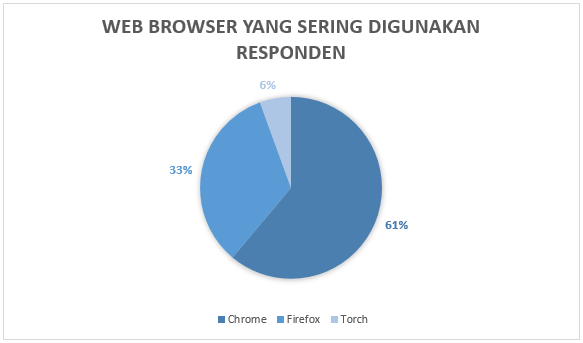
\includegraphics[width=0.9\textwidth,height=0.52\textwidth]
	{pics/webfavorit.PNG}
	\caption{Persentase \f{web browser} yang sering digunakan responden}
	\label{fig:browser}
\end{figure}
\noindent
Gambar \ref{fig:maininet} menjelaskan mengenai persentase rentang penggunaan internet per hari oleh responden. Sebanyak 2 orang (5\%) responden biasa menggunakan internet 1-3 jam per hari, 10 orang (28\%) responden menggunakan internet 3-5 jam per hari, 6 orang (17\%) responden menggunakan 5-7 jam per hari dan 18 orang (50\%) responden menggunakan internet lebih dari 7 jam. Gambar \ref{fig:browser} menunjukan mengenai persentase \f{web browser} yang sering digunakan oleh responden. Terdapat 22 orang (61\%) responden yang biasa menggunakan \f{web browser Google Chrome}, 12 orang (33\%) responden biasa menggunakan \f{web browser Mozilla Firefox} dan 2 orang (6\%) responden biasa menggunakan \f{web browser Torch}.
\begin{figure}
	\centering
	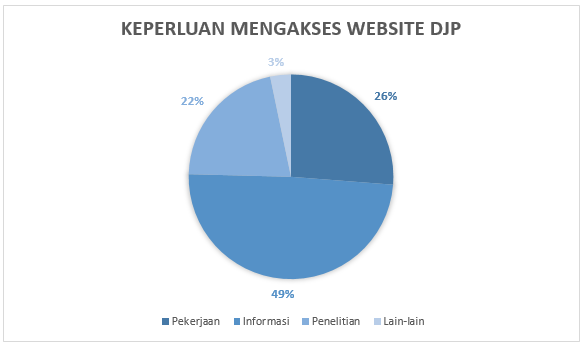
\includegraphics[width=0.9\textwidth,height=0.52\textwidth]
	{pics/keperluanAkses.PNG}
	\caption{Persentase keperluan akses \f{website} DJP Indonesia}
	\label{fig:akses}
\end{figure}
\noindent
Dari data penelitian diketahui bahwa semua responden pernah mengakses \f{website} Direktorat Jenderal Pajak (DJP) Indonesia. Gambar \ref{fig:akses} menjelaskan mengenai persentase keperluan responden mengakses \f{website} Direktorat Jenderal Pajak (DJP) Indonesia. Sebanyak 49\% responden menyatakan keperluan mereka mengakses \f{website} DJP untuk informasi, 26\% responden menyatakan keperluan akses untuk pekerjaan, 22\% responden menyatakan untuk penelitian dan 3\% responden menyatakan keperluan akses \f{website} DJP untuk hal lain-lain.
%-----------------------------------------------------------------------------%
\section{Uji Validitas dan Reliabilitas}
Pada bagian ini dijelaskan mengenai uji validitas dan reliabilitas dari instrumen kuesioner penelitian yang digunakan oleh penulis.
%-----------------------------------------------------------------------------%
\subsection{Uji Validitas}
Uji validitas dilakukan oleh penulis untuk menguji apakah data instrumen penelitian yang digunakan valid atau tidak, instrumen dalam penelitian ini adalah kuesioner yang digunakan untuk pengumpulan data. Pengujian dilakukan menggunakan metode Cronbach's Alpha, pengujian dilakukan dengan melakukan perbandingan nilai \f{corrected item-total correlation} terhadap taraf signifikansi 0.05 \citep{buku.riduwan}. Berikut merupakan kriteria dari pengujian ini.
\begin{itemize}
	\item Bernilai valid jika nilai dari \f{corrected item-total correlation value} (r hitung)  $\geq$ r tabel \f{product moment} dengan derajat kebebasan N-1.
	\item Bernilai tidak valid jika nilai dari \f{corrected item-total correlation value} (r hitung)  $\leq$ r tabel \f{product moment} dengan derajat kebebasan N-1.
\end{itemize}
\begin{table}
	\centering
	\caption{Hasil uji validitas terhadap komponen \f{usability heuristic}.}
	\label{tab:ujivaliditasuh}
	\begin{tabular}{c}
		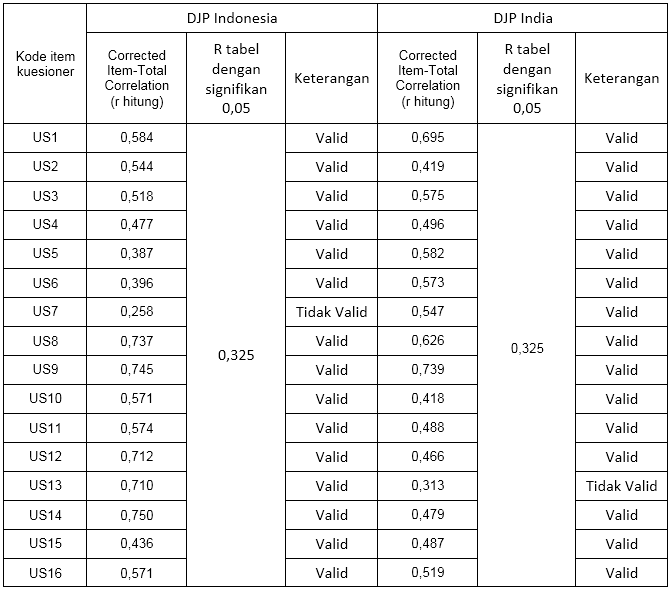
\includegraphics[width=\textwidth]
		{pics/validitasUsabilityHeuristic.PNG}
\end{tabular}
\end{table}
Tabel \ref{tab:ujivaliditasuh} menunjukan bahwa masing-masing data pertanyaan terdapat sebuah nilai yang tidak valid pada komponen \f{usability heuristic} bila dilihat hasil perbandingan r hitung dengan r tabel \f{product moment}. Hal ini disebabkan dari persebaran variatif data yang nilainya kurang signifikan.
\newline\\
Selanjutnya tabel \ref{tab:ujivaliditassat} menerangkan bahwa bahwa semua unit dalam komponen kepuasan pengguna memiliki data yang sudah valid. Nilai pada kolom r-hitung bila dibandingkan denga r-tabel bernilai lebih besar sehingga nilai data valid.
\begin{table}
	\centering
	\caption{Hasil uji validitas terhadap komponen kepuasan pengguna.}
	\label{tab:ujivaliditassat}
	\begin{tabular}{c}
		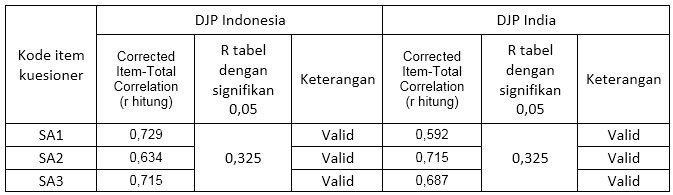
\includegraphics[width=\textwidth]
		{pics/validitasKepuasanPengguna.PNG}
	\end{tabular}
\end{table}
\noindent
Pada tabel \ref{tab:ujivaliditasgq} dapat dilihat nilai r-hitung dari data yang terdapat pada komponen \f{g-Quality} yang ternyata setelah dibandingkan dengan r-tabel terdapat dua buah data yang tidak valid baik di data pengujian DJP Indonesia maupun DJP India.
\begin{table}
	\centering
	\caption{Hasil uji validitas terhadap komponen \f{g-Quality}.}
	\label{tab:ujivaliditasgq}
	\begin{tabular}{c}
		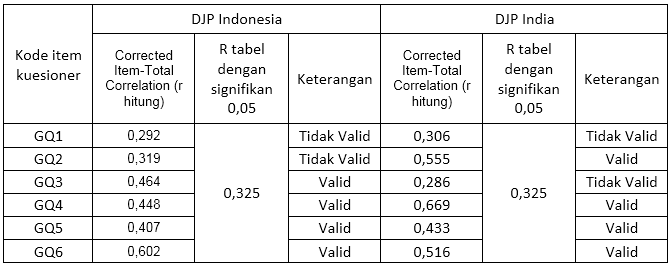
\includegraphics[width=\textwidth]
		{pics/validitasGQuality.PNG}
	\end{tabular}
\end{table}
%-----------------------------------------------------------------------------%
\subsection{Uji Realibilitas}
Uji reliabilitas digunakan untuk menguji instrumen kuesioner yang digunakan pada penelitian terpercaya atau reliabel \citep{article.raharjo}. Uji reliabilitas dilakukan untuk mengetahui tingkat kekonsistenan instrumen kuesioner yang digunakan dalam penelitian. \citet{buku.george} menyatakan bahwa belum ada standar yang mengenai nilai Cronbach's Alpha yang memenuhi nilai acceptable. \citet{buku.george} mambagi nilai dari alpha menjadi 5 bagian dalam tabel \ref{tab:cronalpha} untuk menentukan apakah konsistensi suatu instrumen dapat diterima atau tidak.
\begin{table}
	\centering
	\caption{Kategori Cronbach's Alpha}
	\label{tab:cronalpha}
	\begin{tabular}{|l|l|}
		\hline
		\multicolumn{1}{|c|}{\bf Cronbach's Alpha} & \multicolumn{1}{c|}{{\bf Internal Consistency}} \\ \hline
		a $\geq$ 0.9 & Excellent (High-Stakes testing) \\ \hline
		0.7 $\leq$ a < 0.8 & Good (Low-Stakes testing) \\ \hline
		0.6 $\leq$ a < 0.7 & Acceptable  \\ \hline
		0.5 $\leq$ a < 0.6 & Poor   \\ \hline
		a < 0.5           & Unacceptable  \\ \hline 
	\end{tabular}
		\begin{center}
			{\small Sumber tabel: \citep{buku.george}}
		\end{center}
\end{table}
Tabel \ref{tab:hasilconalp} berikut menunjukan hasil dari uji realibilitas instrumen kuesioner yang digunakan dalam penelitian. Terlihat bahwa komponen pada tiap kuesioner bernilai valid.
\begin{table}
	\centering
	\caption{Hasil penghitungan Cronbach's Alpha terhadap instrumen}
	\label{tab:hasilconalp}
	\begin{tabular}{|l|l|l|l|}
		\cline{2-4}
		\multicolumn{1}{c|}{} &
		\multicolumn{1}{l|}{\bf DJP Indonesia} &
		\multicolumn{1}{l|}{\bf DJP India} &
		\multicolumn{1}{l|}{{\bf Keterangan}} \\ \hline
		\f{Usability Heuristic} & 0,894
		 & 0,879 & Valid \\ \hline
		\f{Satisfaction} & 0,828
		& 0,812 & Valid \\ \hline
		\f{g-Quality} & 0,687
		 & 0,712 & Valid \\ \hline
	\end{tabular}
\end{table}
%-----------------------------------------------------------------------------%
\section{Analisis Data}
Pada bagian ini dijelaskan hasil penghitungan analisis data yang didapat dari instrumen dengan menggunakan aplikasi perangkat lunak SPSS 22. Analisis dilakukan dengan metode \f{paired samples T-test} bila data terdistribusi secara normal, namun jika data tidak terdistribusi secara normal maka digunakan metode \f{Wilcoxon Signed-Rank Test} untuk melihat nilai signifikansi hasil perbandingan.
%-----------------------------------------------------------------------------%
\subsection{\f{Usability Heuristic}}
Pada bagian ini tabel \ref{tab:descuh} menjelaskan bahwa nilai \f{mean} komponen \f{usability heuristic} pada \f{website} DJP India lebih besar dibandingkan dengan \f{website} DJP Indonesia. \f{Website} DJP Indonesia memiliki nilai \f{mean} 4,39409 sedangkan \f{website} DJP India memiliki nilai \f{mean} sebesar 5,42187. Selain nilai \f{mean}, tabel \ref{tab:descuh} juga menunjukan nilai \f{skewness} dan \f{kurtosis} dari masing-masing \f{website} pada komponen \f{usability heuristic}. Maka dapat diketahui nilai dari rasio \f{skewness} dan \f{kurtosis} pada kedua \f{website} tersebut. Nilai rasio \f{skewness} pada \f{website} DJP Indonesia adalah sebesar -0,182/0,393 = -0,4631 dan rasio \f{kurtosis}-nya adalah -0,35/0,768 = -1,0872, sedangkan pada \f{website} DJP India nilai rasio skewnes adalah -0,538/0,393 = -1,3689 dan nilai rasio \f{kurtosis}nya adalah 0,812/0,768 = 1,0572. Telah diketahui bahwa keempat nilai tersebut berada pada rentang -2 dan 2, sehingga dapat disimpulkan bahwa data terdistribusi secara normal. 
\begin{table}
	\centering
	\caption{Hasil statistik deskriptif terhadap komponen \f{usability heuristic}.}
	\label{tab:descuh}
	\begin{tabular}{c}
		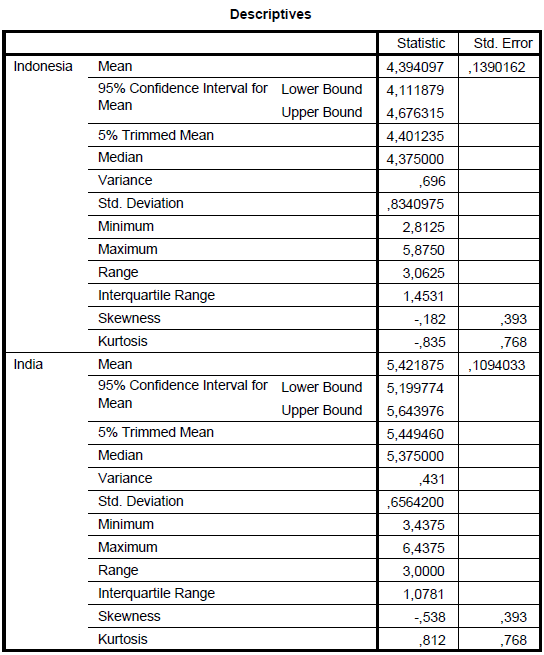
\includegraphics[width=\textwidth]
		{pics/ordinalDescUH.PNG}
	\end{tabular}
\end{table}
\noindent
Diketahui bahwa data terdistribusi secara normal, maka syarat \f{paired samples T-test} telah terpenuhi. Maka dilakukan penghitungan perbandingan nilai kedua \f{website} pada komponen \f{usability heuristic} sehingga diperoleh nilai seperti pada tabel \ref{tab:ttestuh}. Terlihat bahwa hasil \f{paired samples T-test} dalam tabel memiliki nilai signifikansi (Sig. (2-\f{tailed})) untuk komponen \f{usability heuristic} pada \f{website} DJP Indonesia dan India adalah 0,000 (\f{p} < 0,05), sehingga dapat disimpulkan bahwa \textbf{terdapat perbedaan yang signifikan pada komponen \f{usability heuristic} antara \f{website} DJP Indonesia dan DJP India}. Sehingga diketahui bahwa kualitas \f{usability} pada \f{website} DJP India terjaga dengan baik.
\begin{table}[h]
	\centering
	\caption{Hasil \f{paired samples T-test} terhadap komponen \f{usability heuristic}.}
	\label{tab:ttestuh}
	\begin{tabular}{c}
		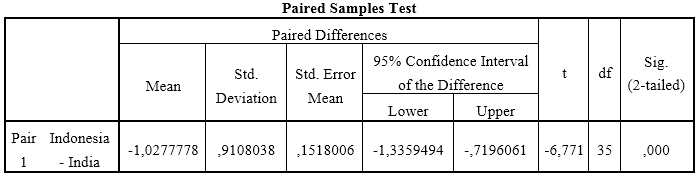
\includegraphics[width=\textwidth]
		{pics/ordinalT-testUH.PNG}
	\end{tabular}
\end{table}
Nilai \f{usability heuristic} pada \f{website} DJP India lebih tinggi dibandingkan dengan \f{website} DJP Indonesia, terlihat dari hasil \f{mean} pada tabel \ref{tab:rata2unituh} penilaian komponen \f{usability heuristic} \f{website} DJP India mendominasi dalam semua unit. Untuk lebih jelas perbandingan nilai \f{mean} setiap unit usablity heuristic, dapat dilihat histogram pada gambar \ref{fig:historata2uh}.
\begin{table}
	\centering
	\caption{Rata-rata nilai unit pada komponen \f{usability heuristic}}
	\label{tab:rata2unituh}
	\resizebox{\textwidth}{!}{%
		\begin{tabular}{ >{\centering\arraybackslash}m{1in} | >{\centering\arraybackslash}m{1in} | >{\centering\arraybackslash}m{1in} | >{\centering\arraybackslash}m{1in} |
				>{\centering\arraybackslash}m{1in} |
				>{\centering\arraybackslash}m{1in} |
				>{\centering\arraybackslash}m{1in} |
				>{\centering\arraybackslash}m{1in} |
				>{\centering\arraybackslash}m{1in} |
				>{\centering\arraybackslash}m{1in} |
				>{\centering\arraybackslash}m{1in} |
			}
			\cline{2-11}
			& UH1        & UH2        & UH3       & UH4       & UH5       & UH6       & UH7       & UH8       & UH9       & UH10 \\
			\hline
			\multicolumn{1}{|l|}{Indonesia} & 4,7777778 & 5,1388889 & 4,75     & 4,555556 & 3,916667 & 4,430556 & 4,87037  & 3,625    & 3,166667 & 4,2222222 \\
			\hline
			\multicolumn{1}{|l|}{India}     & 5,7222222 & 5,5555556 & 4,805556 & 5,361111 & 5,444444 & 5,375    & 5,425926 & 5,555556 & 5,305556 & 5,4166667 \\
			\hline
		\end{tabular}
	}
\end{table}

\begin{figure}
	\centering
	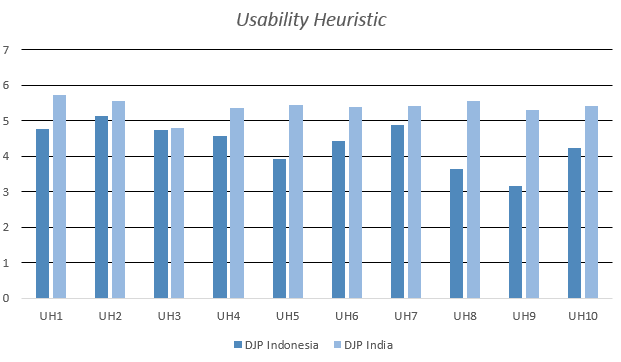
\includegraphics[width=\textwidth]
	{pics/historata2uh.PNG}
	\caption{Histogram \f{mean} unit pada komponen \f{usability heuristic}}
	\label{fig:historata2uh}
\end{figure}
\noindent
Keterangan tabel \ref{tab:rata2unituh} dan gambar \ref{fig:historata2uh}: \\
DJP Indonesia = \f{Website} Direktorat Jenderal Pajak Indonesia
DJP India = \f{Website} Direktorat Jenderal Pajak India
UH1 = \f{Visibility of system status} \\
UH2 = \f{Match between system and real world} \\
UH3 = \f{User control} \\
UH4 = \f{Consistency and standards} \\
UH5 = \f{Error prevention} \\
UH6 = \f{Recognition rather than recall} \\
UH7 = \f{Flexibility and efficiency of use} \\
UH8 = \f{Aesthetic and minimalist design} \\
UH9 = \f{Help user recognize, diagnose and recover from error} \\
UH10 = \f{Help and documentation}
%-----------------------------------------------------------------------------%
\subsection{Kepuasan Pengguna}
Tabel \ref{tab:descsat} menjelaskan bahwa nilai \f{mean} untuk komponen kepuasan pengguna \f{website} DJP India lebih unggul dibanding \f{website} DJP Indonesia. Hal tersebut dapat dilihat dengan nilai \f{mean} \f{website} DJP India yang bernilai 5,3611, sedangkan \f{website} DJP Indonesia memiliki nilai sebesar 4,6111. Selain nilai \f{mean}, dapat diketahui juga dari tabel \ref{tab:descsat} bahwa nilai rasio \f{skewness} untuk \f{website} DJP India adalah 0,070/0,393 = 0,17811 dan rasio \f{kurtosis}-nya -0,664/0,768 = 0,86458. Sedangkan untuk \f{website} DJP Indonesia diketahui bahwa rasio \f{skewness} sebesar -0,365/0,393 = -0,92875 dan rasio \f{kurtosis}-nya 0,309/0,768 = 0,40234. Dengan demikian diketahui bahwa nilai rasio \f{skewness} dan rasio \f{kurtosis} pada masing-masing komponen tingkat kepuasan pengguna terdistribusi secara normal karena terdapat pada rentang -2 dan 2. 
\begin{table}
	\centering
	\caption{Hasil statistik deskriptif terhadap komponen kepuasan pengguna}
	\label{tab:descsat}
	\begin{tabular}{c}
		\includegraphics[width=\textwidth]
		{pics/ordinaldescSAT.PNG}
	\end{tabular}
\end{table}
\noindent
Tabel \ref{tab:ttestsat} menunjukkan bahwa hasil analisa dengan metode \f{paired samples T-test} menunjukan bahwa komponen kepuasan pengguna memiliki nilai yang cukup signifikan dengan nilai signifikansi sebesar 0,003 (\f{p} < 0,05). Ini menunjukkan bahwa komponen tingkat kepuasan pengguna saat menggunakan \f{website} DJP Indonesia dan India \textbf{memiliki perbedaan yang signifikan}. Dari hasil tersebut diketahui bahwa kualitas \f{usability} dari DJP Indonesia kurang terjaga, hal tersebut dapat dilihat dari perbandingan \f{mean} tingkat kepuasan pengguna.
\begin{table}
	\centering
	\caption{Hasil \f{paired samples T-test} terhadap komponen kepuasan pengguna}
	\label{tab:ttestsat}
	\begin{tabular}{c}
		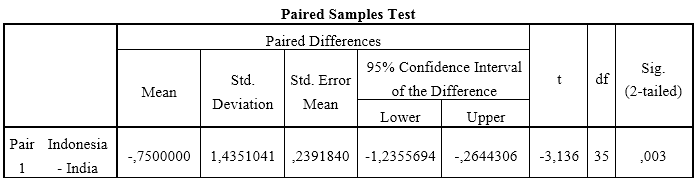
\includegraphics[width=\textwidth]
		{pics/ordinalT-testSAT.PNG}
	\end{tabular}
\end{table}
\noindent
%-----------------------------------------------------------------------------%
\subsection{Komponen \f{g-Quality}}
Pada tabel \ref{tab:descgq} dijelaskan bahwa nilai \f{mean} komponen \f{g-quality} pada \f{website} DJP India lebih besar dibandingkan dengan \f{website} DJP Indonesia. \f{Website} DJP Indonesia memiliki nilai \f{mean} 4,1111 sedangkan \f{website} DJP India memiliki nilai \f{mean} sebesar 5,2870. Selain nilai \f{mean}, tabel \ref{tab:descgq} juga menunjukan nilai \f{skewness} dan \f{kurtosis} dari masing-masing \f{website} pada komponen \f{g-quality}. Maka diketahui nilai rasio \f{skewness} dan \f{kurtosis} pada kedua \f{website} tersebut. Nilai rasio \f{skewness} pada \f{website} DJP Indonesia adalah sebesar -0,554/0,393 = -1,4096 dan rasio \f{kurtosis} sebesar -0,747/0,768 = -0,9726, pada \f{website} DJP India nilai rasio skewnes adalah -0,638/0,393 = -1,6324 dan nilai rasio \f{kurtosis}nya adalah 1,361/0,768 = 1,7721. Jelas bahwa keempat nilai tersebut berada pada rentang -2 dan 2, sehingga dapat disimpulkan bahwa data terdistribusi secara normal. 
\begin{table}
	\centering
	\caption{Hasil statistik deskriptif terhadap komponen \f{g-Quality}}
	\label{tab:descgq}
	\begin{tabular}{c}
		\includegraphics[width=\textwidth]
		{pics/ordinaldescGQ.PNG}
	\end{tabular}
\end{table}
\noindent
Setelah diketahui data terdistribusi secara normal, maka analisa \f{paired samples T-test} dilakukan untuk penghitungan perbandingan nilai kedua \f{website} pada komponen \f{g-quality} sehingga diperoleh nilai seperti pada tabel \ref{tab:ttestgq}. Terlihat bahwa hasil \f{paired samples T-test} dalam tabel memiliki nilai signifikansi (Sig. (2-\f{tailed})) untuk komponen \f{g-quality} pada \f{website} DJP Indonesia dan India adalah 0,000 (\f{p} < 0,05), sehingga dapat disimpulkan bahwa \textbf{terdapat perbedaan yang signifikan pada komponen \f{g-quality} antara \f{website} DJP Indonesia dan DJP India}. Sehingga diketahui bahwa kualitas \f{usability} pada \f{website} DJP India terjaga baik.
\begin{table}
	\centering
	\caption{Hasil \f{paired samples T-test} terhadap komponen \f{g-quality}}
	\label{tab:ttestgq}
	\begin{tabular}{c}
		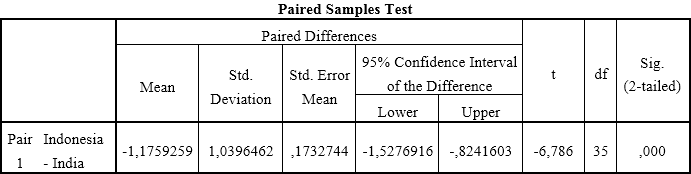
\includegraphics[width=\textwidth]
		{pics/ordinalT-testGQ.PNG}
	\end{tabular}
\end{table}
\noindent
Nilai \f{g-quality} pada \f{website} DJP India lebih tinggi dibandingkan dengan \f{website} DJP Indonesia, terlihat dari hasil \f{mean} pada tabel \ref{tab:rata2unitgq} penilaian komponen \f{g-quality} \f{website} DJP India mendominasi dalam semua unit. Untuk lebih jelas perbandingan nilai \f{mean} setiap unit usablity heuristic, dapat dilihat histogram pada gambar \ref{fig:historata2gq}.
\begin{table}
	\centering
	\caption{Rata-rata nilai unit pada komponen \f{g-quality}}
	\label{tab:rata2unitgq}
	\resizebox{\textwidth}{!}{%
		\begin{tabular}{ >{\centering\arraybackslash}m{1in} | >{\centering\arraybackslash}m{1in} | >{\centering\arraybackslash}m{1in} | >{\centering\arraybackslash}m{1in} |
				>{\centering\arraybackslash}m{1in} |
				>{\centering\arraybackslash}m{1in} |
				>{\centering\arraybackslash}m{1in} |
			}
			\cline{2-7}
			& GQ1        & GQ2        & GQ3       & GQ4       & GQ5       & GQ6  \\
			\hline
			\multicolumn{1}{|l|}{Indonesia} & 3,944444444 & 4,333333333 & 3,833333333 & 4,5 & 4 & 4,055555556 \\ \hline
			\multicolumn{1}{|l|}{India}     & 4,444444444 & 5,472222222 & 5,611111111 & 5,527777778 & 5,527777778 & 5,138888889 \\ \hline
		\end{tabular}
	}
\end{table}

\begin{figure}
	\centering
	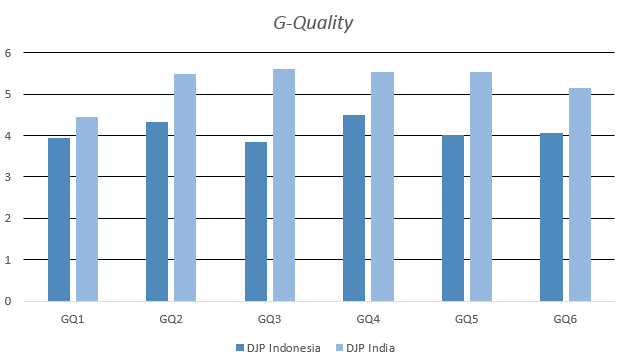
\includegraphics[width=\textwidth]
	{pics/historata2gq.PNG}
	\caption{Histogram \f{mean} unit pada komponen \f{g-quality}}
	\label{fig:historata2gq}
\end{figure}
\pagebreak

\noindent
Keterangan tabel \ref{tab:rata2unitgq} dan gambar \ref{fig:historata2gq}: \\
DJP Indonesia = \f{Website} Direktorat Jenderal Pajak Indonesia
DJP India = \f{Website} Direktorat Jenderal Pajak India
GQ1 = \f{Accessibility} \\
GQ2 = \f{Interoperability} \\
GQ3 = \f{Security and privacy} \\
GQ4 = \f{Information reliability} \\
GQ5 = \f{Service agility} \\
GQ6 = \f{Transparency} \\
%-----------------------------------------------------------------------------%
\subsection{Efisiensi}
Efisiensi dapat diukur dengan mengukur berapa banyak waktu yang digunakan oleh responden untuk menyelesaikan tugas yang diberikan, seperti yang telah dijelaskan sebelumnya pada subbab \ref{subsec:usability}. Diketahui dari tabel \ref{tab:descwaktu} bahwa \f{mean} lama waktu pengerjaan tugas pada \f{website} DJP Indonesia lebih besar dibandingkan dengan \f{website} DJP India. \f{Website} DJP Indonesia memiliki \f{mean} waktu selama 755,94 detik, sedangkan \f{website} DJP India memiliki \f{mean} waktu selama 670,13. Selain \f{mean} waktu pengerjaan tugas, tabel \ref{tab:descwaktu} juga menunjukan nilai \f{skewness} dan \f{kurtosis} dari masing-masing \f{website} pada lama waktu pengerjaan tugas. Maka diketahui nilai rasio \f{skewness} dan \f{kurtosis} pada kedua \f{website} tersebut. Nilai rasio \f{skewness} pada \f{website} DJP Indonesia adalah sebesar 0,601/0,393 = 1,529 dan rasio \f{kurtosis} sebesar -0,869/0,768 = -1,131, pada \f{website} DJP India nilai rasio skewnes adalah 0,424/0,393 = 1,078 dan nilai rasio \f{kurtosis}nya adalah -0,971/0,768 = -1,264. Jelas bahwa keempat nilai tersebut berada pada rentang -2 dan 2, sehingga dapat disimpulkan bahwa data terdistribusi secara normal. 
\begin{table}
	\centering
	\caption{Hasil statistik deskriptif terhadap lama waktu pengerjaan tugas}
	\label{tab:descwaktu}
	\begin{tabular}{c}
		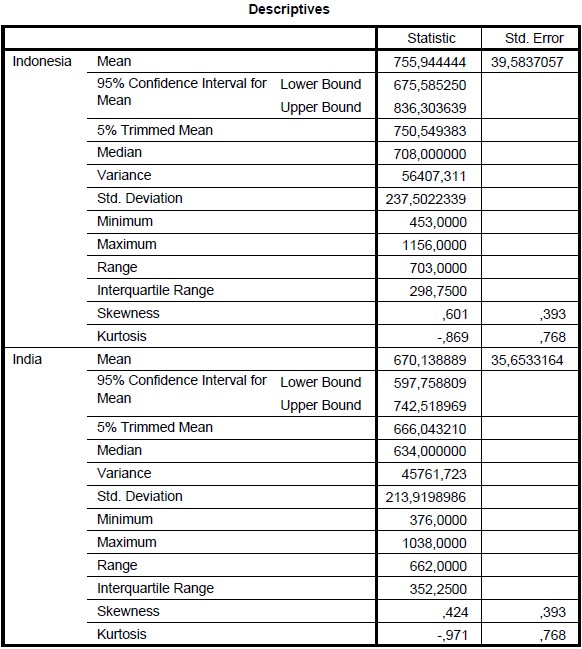
\includegraphics[width=\textwidth]
		{pics/waktudesc.PNG}
	\end{tabular}
\end{table}
\noindent
Setelah diketahui data terdistribusi secara normal, maka analisa \f{paired samples T-test} dilakukan untuk penghitungan perbandingan nilai kedua \f{website} pada lama waktu pengerjaan tugas sehingga diperoleh nilai seperti pada tabel \ref{tab:ttestwaktu}. Terlihat bahwa hasil \f{paired samples T-test} dalam tabel memiliki nilai signifikansi (Sig. (2-\f{tailed})) untuk lama waktu pengerjaan tugas pada \f{website} DJP Indonesia dan India adalah 0,000 (\f{p} < 0,05), sehingga dapat disimpulkan bahwa \textbf{terdapat perbedaan yang signifikan terhadap lama waktu pengerjaan tugas antara \f{website} DJP Indonesia dan DJP India}. Sehingga diketahui bahwa responden lebih banyak menghabiskan waktu pada \f{website} DJP Indonesia walau sesungguhnya \f{website} DJP India menggunakan bahasa yang bukan bahasa utama di negara Indonesia, selain itu \f{website} DJP Indonesia memuat banyak konten dalam satu halaman sehingga membuat bingung responden untuk mencari menu dan tugas yang dimaksud.
\begin{table}
	\centering
	\caption{Hasil \f{paired samples T-test} terhadap lama waktu pengerjaan tugas}
	\label{tab:ttestwaktu}
	\begin{tabular}{c}
		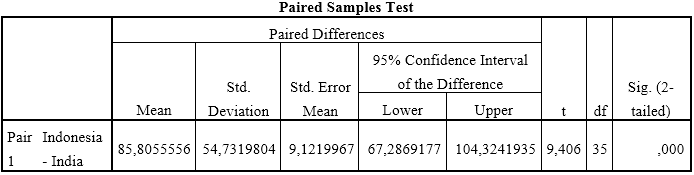
\includegraphics[width=\textwidth]
		{pics/waktuSelesaiT-test.PNG}
	\end{tabular}
\end{table}
%-----------------------------------------------------------------------------%
\subsection{Efektivitas}
Efektivitas dapat diukur dengan menghitung keberhasilan pengguna dalam mengerjakan tugas yang diberikan. Pada tabel \ref{tab:desctugasselesai} terlihat bahwa \f{mean} tugas yang berhasil dikerjakan pada \f{website} DJP India lebih banyak dibandingkan dengan \f{website} DJP Indonesia. \f{Website} DJP Indonesia memiliki \f{mean} tugas yang berhasil dikerjakan sebanyak 9,5833, sedangkan \f{website} DJP India memiliki \f{mean} tugas berhasil dikerjakan sebanyak 9,6944. Selain \f{mean} tugas yang berhasil dikerjakan, tabel \ref{tab:desctugasselesai} juga menunjukan nilai \f{skewness} dan \f{kurtosis} dari masing-masing \f{website} dalam tugas yang berhasil dikerjakan. Maka diketahui nilai rasio \f{skewness} dan \f{kurtosis} pada kedua \f{website} tersebut. Nilai rasio \f{skewness} pada \f{website} DJP Indonesia adalah sebesar -2,213/0,393 = -5,631 dan rasio \f{kurtosis} sebesar 3,823/0,768 = 4,977, pada \f{website} DJP India nilai rasio skewnes adalah -2,520/0,393 = -6,412 dan nilai rasio \f{kurtosis}nya adalah 6,123/0,768 = 8,024. Dari data sebelumnya terlihat bahwa keempat nilai tersebut tidak berada pada rentang -2 dan 2, sehingga dapat disimpulkan bahwa data tidak terdistribusi secara normal. Dikarenakan data yang tidak terdistribusi normal maka dilakukan transformasi dan pengujian ulang, namun data masih tetap tidak terdistribusi secara normal. Setelah mengetahui bahwa data tidak dapat ditransformasi maka digunakan penghitungan perbandingan non-parametrik menggunakan metode \f{Wilcoxon Signed Rank Test} sebagai pengganti \f{paired samples T-test}.
\begin{table}
	\centering
	\caption{Hasil statistik deskriptif terhadap tugas yang berhasil dikerjakan}
	\label{tab:desctugasselesai}
	\begin{tabular}{c}
		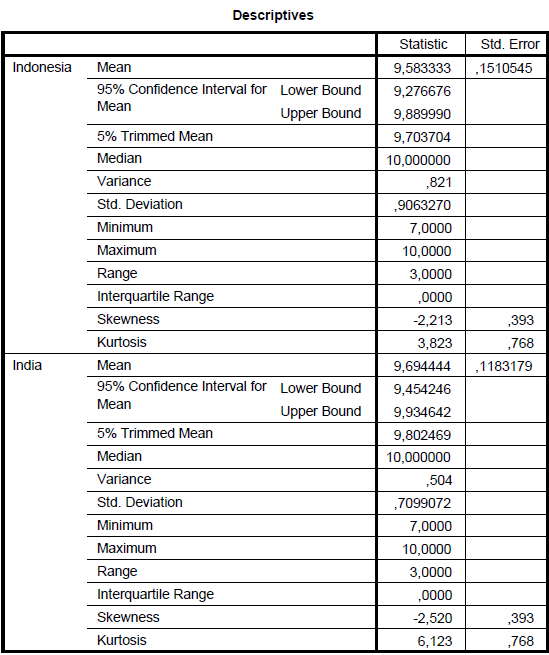
\includegraphics[width=\textwidth]
		{pics/tugasselesaidesc.PNG}
	\end{tabular}
\end{table}
Terlihat bahwa hasil \f{wilcoxon signed rank test} dalam tabel \ref{tab:hasiltugasselesai} memiliki nilai signifikansi (Sig. (2-\f{tailed})) untuk tugas yang berhasil dikerjakan pada \f{website} DJP Indonesia dan India adalah 0,285 (\f{p} > 0,05), sehingga dapat disimpulkan bahwa \textbf{tidak terdapat perbedaan yang signifikan antara jumlah tugas yang berhasil dikerjakan pada \f{website} DJP Indonesia dan DJP India}. Sehingga diketahui bahwa responden hampir sama banyaknya menyelesaikan tugas dalam pengujian \f{website} DJP Indonesia dengan DJP India.
\begin{table}
	\centering
	\caption{Rank \f{wilcoxon signed rank test} terhadap tugas yang berhasil dikerjakan}
	\label{tab:ranktugasselesai}
	\begin{tabular}{c}
		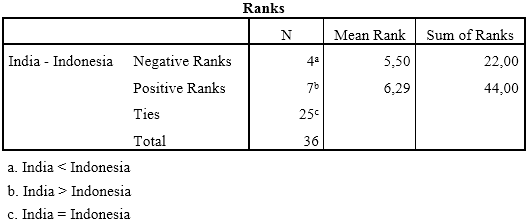
\includegraphics[width=\textwidth]
		{pics/rankSelesai.PNG}
	\end{tabular}
\end{table}
\begin{table}
	\centering
	\caption{Hasil \f{wilcoxon signed rank test} terhadap tugas yang berhasil dikerjakan}
	\label{tab:hasiltugasselesai}
	\begin{tabular}{c}
		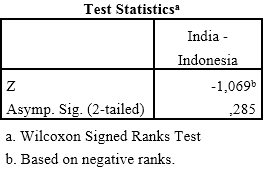
\includegraphics[width=0.5\textwidth]
		{pics/selesaiWilcoxon.PNG}
	\end{tabular}
\end{table}
%-----------------------------------------------------------------------------%
\subsection{Tingkat Kesalahan Pengguna}
Pengukuran tingkat kelasahan pengguna dilakukan dengan melakukan pencatatan terhadap pengerjaan tugas yang gagal dilakukan oleh pengguna pada pengujian \f{website} DJP Indonesia dengan India. Pada tabel \ref{tab:tugasgagaldesc} terlihat bahwa \f{mean} kesalahan yang dilakukan pengguna pada \f{website} DJP Indonesia lebih banyak dibandingkan dengan \f{website} DJP India. \f{Website} DJP Indonesia memiliki \f{mean} tugas yang gagal dikerjakan sebanyak 0,4166, sedangkan \f{website} DJP India memiliki \f{mean} tugas yang gagal dikerjakan sebanyak 0,0653. Selain \f{mean} tugas yang gagal dikerjakan, tabel \ref{tab:desctugasselesai} juga menunjukan nilai \f{skewness} dan \f{kurtosis} dari masing-masing \f{website} dalam tugas yang gagal dikerjakan. Maka diketahui nilai rasio \f{skewness} dan \f{kurtosis} pada kedua \f{website} tersebut. Nilai rasio \f{skewness} pada \f{website} DJP Indonesia adalah sebesar 2,213/0,393 = 5,631 dan rasio \f{kurtosis} sebesar 3,823/0,768 = 4,977, pada \f{website} DJP India nilai rasio skewnes adalah 2,520/0,393 = 6,412 dan nilai rasio \f{kurtosis}nya adalah 6,123/0,768 = 8,024. Dari data sebelumnya terlihat bahwa keempat nilai tersebut tidak berada pada rentang -2 dan 2, sehingga dapat disimpulkan bahwa data tidak terdistribusi secara normal. Dikarenakan data yang tidak terdistribusi normal maka dilakukan transformasi dan pengujian ulang, namun data masih tetap tidak terdistribusi secara normal. Setelah mengetahui bahwa data tidak dapat ditransformasi maka digunakan penghitungan perbandingan non-parametrik menggunakan metode \f{Wilcoxon Signed Rank Test} sebagai pengganti \f{paired samples T-test}.
\begin{table}
\centering
\caption{Hasil statistik deskriptif terhadap tugas yang gagal dikerjakan responden}
\label{tab:tugasgagaldesc}
\begin{tabular}{c}
	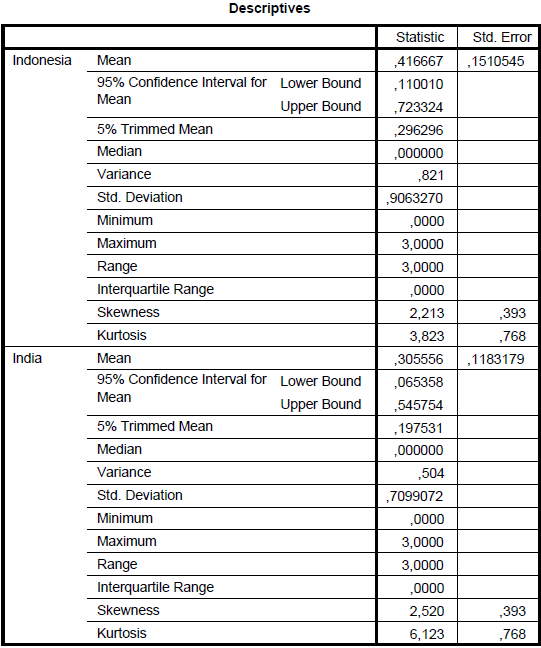
\includegraphics[width=\textwidth]
	{pics/tugasgagaldesc.PNG}
\end{tabular}
\end{table}
\noindent
Terlihat bahwa hasil \f{wilcoxon signed rank test} dalam tabel \ref{tab:hasiltugasgagal} memiliki nilai signifikansi (Sig. (2-\f{tailed})) untuk tugas yang gagal dikerjakan pada \f{website} DJP Indonesia dan India adalah 0,285 (\f{p} > 0,05), sehingga dapat disimpulkan bahwa \textbf{tidak terdapat perbedaan yang signifikan antara jumlah kesalahan yang dilakukan pengguna ketika menggunakan \f{website} DJP Indonesia dan DJP India}. Sehingga diketahui bahwa responden tidak terlalu banyak gagal menyelesaikan tugas dalam pengujian \f{website} DJP Indonesia dengan DJP India. Dari hasil observasi kesalahan yang terjadi dikarenakan penggunaan istilah yang tidak umum digunakan.
\begin{table}
	\centering
	\caption{Rank \f{wilcoxon signed rank test} terhadap tugas yang berhasil dikerjakan responden}
	\label{tab:ranktugasgagal}
	\begin{tabular}{c}
		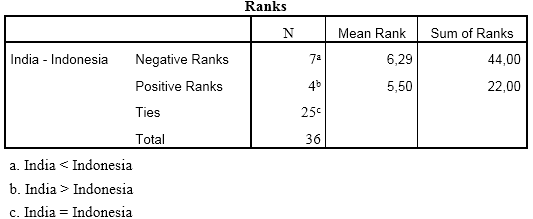
\includegraphics[width=\textwidth]
		{pics/rankGagal.PNG}
	\end{tabular}
\end{table}
\begin{table}
	\centering
	\caption{Hasil \f{wilcoxon signed rank test} terhadap tugas yang berhasil dikerjakan responden}
	\label{tab:hasiltugasgagal}
	\begin{tabular}{c}
		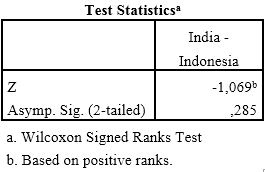
\includegraphics[width=0.5\textwidth]
		{pics/gagalWilcoxon.PNG}
	\end{tabular}
\end{table}
%-----------------------------------------------------------------------------%
\subsection{Preferensi Pengguna}
Dari hasil \f{open ended question} yang penulis berikan kepada responden terkait preferensi pengguna dalam menilai \f{website} DJP Indonesia dan India yang dibandingkan maka diperoleh hasil seperti pada gambar \ref{fig:preferensigraf}. Pada grafike gambar \ref{fig:preferensigraf} terlihat bahwa responden lebih cenderung memilih \f{website} DJP India.
Adapun beberapa alasan yang dikemukakan oleh responden memilih \f{website} DJP India sehingga menjadi dasar penilaian dengan penarikan kesimpulan sebagai berikut.
\begin{enumerate}
	\item Tampilan \f{website} DJP India lebih sederhana segingga mudah dimengerti dan digunakan, selain itu tampilan menarik karena banyak memberikan konten yang informatif.
	\item {Website} DJP India lebih mudah digunakan karena aksesnya cepat.
	\item Keamanan lebih baik pada \f{website} DJP India
	\item Penelusuran konten lebih mudah, sehingga pengguna merasa terbantu dan mudah mencari informasi yang dituju.
\end{enumerate}
Selain alasan memilih \f{website} DJP India diatas terdapat juga alasan terkait responden yang memilih \f{website} DJP Indonesia sebagai berikut.
\begin{enumerate}
	\item Sudah terbiasa menggunakan \f{website} DJP Indonesia.
	\item Fitur \f{e-filling} DJP Indonesia lebih bagus daripada DJP India.
	\item Konten yang dimiliki banyak.
\end{enumerate}

\begin{figure}
	\centering
	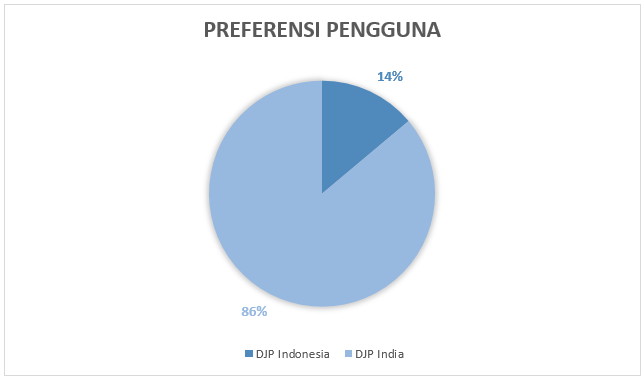
\includegraphics[width=\textwidth]
	{pics/preferensipengguna.PNG}
	\caption{Grafik preferensi pengguna terhadap \f{website} DJP Indonesia dan India}
	\label{fig:preferensigraf}
\end{figure}
\pagebreak
%-----------------------------------------------------------------------------%
\subsection{Analisa Perbandingan Teori}
Setelah mengetahui hasil analisa dari analisis perbandingan \f{usability testing} dan teori yang dikemukakan pada subbab \ref{subsec:gquality}. Maka dilakukan perbandingan penilaian \f{usability heuristic} dan \f{g-quality} berdasar lima kriteria evaluasi \f{e-government} sebagai berikut.
\begin{enumerate}
	\item \f{Cognitive Effort}\\
	Terlihat pada tabel \ref{tab:kriteriaegov} nilai yang dimiliki oleh \f{website} DJP Indonesia lebih rendah dari \f{website} DJP India. Penilaian cognitive effort didapat berdasarkan pencarian nilai dari penggolongan kriteria berdasarkan tabel \ref{tab:mappingegov}. Diketahui bahwa kedua \f{website} \f{e-government} memiliki nilai yang cukup berbeda, dimana \f{website} DJP Indonesia memiliki skor evaluasi sebesar \textbf{61,56} yang tergolong \textbf{cukup baik}, sedangkan \f{website} DJP India memiliki nilai sebesar \textbf{75,86} yang tergolong ke nilai yang \textbf{baik}. Sehingga dapat dijelaskan bahwa untuk mengakses \f{website} DJP Indonesia diperlukan usaha lebih untuk memahami terkait aspek kognitif dan menyesuaikan kebutuhan penggunaan sehingga pengguna harus mempelajari \f{website} agar dapat menggunakannya dengan lancar.
	\item \f{Tolerance}\\
	Pada tabel \ref{tab:kriteriaegov} terdapat perbedaan yang cukup signifikan pada kriteria toleransi untuk \f{website} DJP Indonesia dibanding India. Evaluasi terhadap kriteria ini menunjukkan bahwa \f{website} DJP Indonesia memiliki skor sebesar \textbf{58,36} yang digolongkan sebagai nilai yang \textbf{cukup}, sedangkan \f{website} DJP India mendapatkan skor \textbf{76,47} yang tergolong sebagai nilai \textbf{baik}. Hal ini menunjukkan bahwa \f{website} DJP Indonesia belum memberikan toleransi yang memuaskan terhadap pengguna yang dengan sabar menunggu, memahami dan melakukan aktivitas sesuai dengan respon dari \f{website}. 
	\item \f{Reach}\\
	Tabel \ref{tab:kriteriaegov} menunjukkan bahwa perbedaan nilai skor hasil evaluasi \f{usability} \f{e-government} antara \f{website} DJP Indonesia dan India memiliki jarak skor kriteria keterjangkauan yang paling dekat walau masih terpaut jauh dalam jumlah skor. Evaluasi terhadap kriteria ini menunjukkan bahwa \f{website} DJP Indonesia memiliki skor sebesar \textbf{63,39} yang tergolong \textbf{cukup baik}, sedangkan \f{website} DJP India memiliki skor sebesar \textbf{75,30} yang tergolong \textbf{baik}. Dengan demikian diketahui bahwa \f{website} DJP Indonesia masih memiliki kekurangan dalam keterjangkauan \f{website} kepada masyarakat.
	\item \f{Physical Effort}\\
	Pada tabel \ref{tab:kriteriaegov} diketahui bahwa \f{website} DJP Indonesia masih belum ungul dalam kriteria usaha fisik. Tabel \ref{tab:kriteriaegov} menunjukkan bahwa nilai skor hasil evaluasi \f{usability} \f{e-government} \f{website} DJP Indonesia memiliki skor sebesar \textbf{58,91} yang tergolong \textbf{cukup}, sedangkan \f{website} DJP India sebesar \textbf{77,16} yang tergolong \textbf{baik}. Hal ini menunjukkan bahwa \f{website} DJP Indonesia belum mudah untuk digunakan seperti pada hal penggunaan data yang kurang dimanfaatkan secara berulang-ulang.
	\item \f{Trust}\\
	Pada tabel \ref{tab:kriteriaegov} menunjukkan bahwa nilai skor pada kriteria kepercayaan dari \f{website} DJP Indonesia masih lebih rendah dibandingkan dengan \f{website} DJP India. \f{Website} DJP Indonesia memiliki skor sebesar \textbf{58,02} yang tergolong \textbf{cukup}, sedangkan \f{website} DJP India memiliki nilai \textbf{77,86} yang tergolong \textbf{baik}. Hal yang menyebabkan \f{website} DJP Indonesia memiliki nilai yang rendah pada kriteria ini karena masyarakat masih belum mempercayai \f{website} DJP Indonesia, fitur seperti keamanan akun masih dirasa kurang pada \f{website} DJP Indonesia sehingga menunjukkan bahwa \f{website} belum dapat dipercaya.
\end{enumerate}
Tabel \ref{tab:nilaiegov} menunjukkan nilai skor hasil evaluasi \f{usability website e-government} DJP Indonesia dan India per unit. Terlihat pada tabel untuk tiap unit komponen \f{website} DJP India mendominasi penilaian skor.
\begin{table}
	\centering
	\caption{Nilai dari evaluasi \f{usability e-government}}
	\label{tab:nilaiegov}
	\resizebox{\textwidth}{!}{%
		\begin{tabular}{|l|l|l|}
			\hline
			\multicolumn{1}{|c|}{\multirow{2}{*}{Komponen}} & \multicolumn{2}{c|}{Nilai Evaluasi (0$-$100\%)} \\ \cline{2-3} 
			& DJP Indonesia                                 & DJP India                                 \\ \hline
			\f{Visibility of system status} & 68,25 & 81,75 \\ \hline
			\f{Match between system and the real world} & 73,41 & 79,37 \\ \hline
			\f{User control and freedom} & 67,86 & 68,65 \\ \hline
			\f{Consistency and standards} & 65,08 & 76,59 \\ \hline
			\f{Error prevention} & 55,95 & 77,78 \\ \hline
			\f{Recognition rather than recall} & 63,29 & 76,79 \\ \hline
			\f{Flexibility and efficiency of use} & 69,58 & 77,51 \\ \hline
			\f{Aesthetics and minimalist design} & 51,79 & 79,37 \\ \hline
			\f{Help users recognize, diagnose, and recover from errors} & 45,24 & 75,79 \\ \hline
			\f{Help and documentation} & 60,32 & 77,38 \\ \hline
			\f{Accessibility} & 56,35 & 63,49 \\ \hline
			\f{Interoperability} & 61,90 & 78,17 \\ \hline
			\f{Security and privacy} & 54,76 & 80,16 \\ \hline
			\f{Information truth and precision} & 64,29 & 78,97 \\ \hline
			\f{Service Agility} & 57,14 & 78,97 \\ \hline
			\f{Transparency} & 57,94 & 73,41 \\ \hline
		\end{tabular}
	}
\end{table}
\begin{table}
	\centering
	\caption{Nilai evaluasi berdasarkan kriteria \f{e-government}}
	\label{tab:kriteriaegov}
	\begin{tabular}{|l|l|l|}
			\hline
			\multicolumn{1}{|c|}{\multirow{2}{*}{Kriteria}} & \multicolumn{2}{c|}{Nilai Evaluasi (0$-$100\%)} \\ \cline{2-3} 
			& DJP Indonesia                                 & DJP India                                   \\ \hline
			\f{Cognitive Effort}    & 61,56                                   & 75,86                                 \\ \hline
			\f{Tolerance}           & 58,36                                   & 76,47                                  \\ \hline
			\f{Reach}               & 63,39                                   & 75,30                                 \\ \hline
			\f{Physical Effort}     & 58,91                                   & 77,16                                 \\ \hline
			\f{Trust}               & 58,02                                   & 77,86                                 \\ \hline
		\end{tabular}
\end{table}
%-----------------------------------------------------------------------------%
\subsection{Rekomendasi Perbaikan}
Tabel \ref{tab:perbaikan} merupakan tabel rekomendasi perbaikan yang berhasil penulis himpun dari analisis data dan juga rekomendasi yang diberikan oleh responden. Tabel ini dijadikan dasar acuan untuk mengembangkan \f{high-fidelity prototyping}.
\begin{center}

\begin{longtable}{|p{0.5cm}|p{3.8cm}|p{3.8cm}|p{4.2cm}|}
	\caption{Rekomendasi perbaikan untuk \f{website} DJP Indonesia}
	\label{tab:perbaikan} \\
			\hline
			\textbf{No.} & \textbf{Rumusan Perbaikan} & \textbf{\f{Usability Heuristic}} & \textbf{Rekomendasi yang dirangkum dari Responden} \\ \hline \endhead
			1 & Perbaikan halaman \f{homepage} dari website DJP Indonesia agar lebih sederhana, dengan cara menggabungkan ulang menu dan desain ulang halaman. & \f{Aesthetic and minimalist design, match between system and the realworld, consystency and standards} dan \f{flexibility and efficiency of use.} & Perubahan tampilan yang lebih sederhana, rapih dan tata letak yang lebih baik.\\ \hline
			2 & Perbaikan halaman artikel dengan pengelompokkan tipe artikel dan informasi penyajian artikel. & \f{Consystency and standards, flexibility and efficiency of use, recognition rather than recall} dan \f{information truth and precision.} & Perbaiki dan perkaya konten sehingga lebih mudah mendapat informasi. \\ \hline
			3 & Perbaikan halaman \f{error} apabila pengguna melakukan kesalahan, serta halaman penanganannya. & \f{Error prevention, user control} dan \f{help user recognize, diagnose and recover from errors.} & Pemberitahuan terkait kesalahan seperti pencarian  \\ \hline
			4 & Perbaikan halaman download dengan pengelompokkan file yang lebih teratur dan rapih. & \f{Aesthetic and minimalist design, match between system and the realworld, consystency and standards, flexibility and efficiency of use} dan \f{recognition rather than recall.} & Halaman yang lebih rapih lagi.  \\ \hline
			5 & Perbaikan halaman aplikasi sebagai layanan penting yang ditawarkan kepada masyarakat. & \f{Aesthetic and minimalist design, match between system and the realworld, consystency and standards, flexibility and efficiency of use} dan \f{recognition rather than recall.} & Halaman aplikasi disatukan sehingga mudah diakses  \\ \hline
			6 & Perbaikan halaman login dari aplikasi \f{e-filling} untuk meningkatkan struktur keamanan. & \f{Security and privacy} & Perbaiki keamanan website sehingga merasa aman.  \\ \hline
			7 & Perbaikan halaman tutorial dan bentuk FAQ untuk mendukung pembelajaran terkait \f{website} kepada pengguna. & \f{Error prevention, help and documentation} dan \f{accessibility.} & Halaman FAQ dan tutorial yang lebih lengkap lagi. \\ \hline
			8 & Perbaikan halaman yang memberikan informasi terkait pengumuman sehingga memberikan informasi yang lebih akurat, terpercaya dan transparan & \f{Transparency} dan \f{information truth and precision.} & \f{Update} mengenai peraturan dan aturan yang dikelompokkan sehingga tersusun jelas. \\ \hline
			9   & Perbaikan halaman tautan antar \f{website e-government} sehingga aspek \f{interoperability} terpenuhi. & \f{Interoperability}. & Dapat akses informasi dengan website pemerintahan lain. \\ \hline
			10  & Perbaikan halaman layanan informasi sehingga aspek pelayanan lebih baik. & \f{Service agility}. & Informasi yang mudah didapat. \\ \hline
\end{longtable}
\end{center}

%-----------------------------------------------------------------------------%
%-----------------------------------------------------------------------------%
\chapter{\babLima}
%-----------------------------------------------------------------------------%

%-----------------------------------------------------------------------------%
\section{Implementasi \f{Cluster}}
%-----------------------------------------------------------------------------%

%-----------------------------------------------------------------------------%
\subsection{Instalasi \f{Frontend}}
%-----------------------------------------------------------------------------%
Tabel model lain, ditunjukkan pada tabel \ref{tab:infohasti}. 
\begin{table}
	\centering
	\caption{Informasi \f{cluster} X}
	\newcolumntype{g}{>{\columncolor{headertbl}}c}
	\label{tab:infohasti}
	\begin{tabular}{|g|c|}
	\hline Host Name & X\\
	\hline Cluster Name & X\\
	\hline Certificate Organization & UI\\
	\hline Certificate Locality & Depok\\
	\hline Certificate State & West Java\\
	\hline Certificate Country & ID\\
	\hline Contact & X\\
	\hline URL & http://grid.ui.ac.id\\
	\hline
	\end{tabular}
\end{table}

Ada pagebreak disini.
%supaya rapih
\pagebreak

Another type of table
\begin{table}
	\centering
	\caption{Perbandingan Partisi \f{default} dan manual}
	\newcolumntype{g}{>{\columncolor{headertbl}}c}
	\label{tab:partdisk}
	\begin{tabular}{|g|c|c|}
	\rowcolor{headertbl}
	\hline & Partisi default & Partisi manual yang dilakukan\\
	\hline / & 16 GB & 30 GB\\
	\hline /var & 4 GB & 18 GB\\
	\hline swap & 1 GB & 2 GB\\
	\hline /export & 55 GB & 26 GB\\
	\hline
	\end{tabular}
\end{table}

Program menghasilkan keluaran seperti pada kode \ref{lst:raidready}. 

\begin{minipage}{\linewidth}
\begin{lstlisting}[caption={Keluaran output},label={lst:raidready}]
[root@nas-0-0 ~]# cat /proc/mdstat 
Personalities : [raid1] 
md0 : active raid1 sda4[0] sdb2[1]
      1917672312 blocks super 1.2 [2/2] [UU]
      
unused devices: <none>
[root@nas-0-0 ~]# mdadm --detail /dev/md0 
/dev/md0:
        Version : 1.2
  Creation Time : Fri May  3 15:38:52 2013
     Raid Level : raid1
     Array Size : 1917672312 (1828.83 GiB 1963.70 GB)
  Used Dev Size : 1917672312 (1828.83 GiB 1963.70 GB)
   Raid Devices : 2
  Total Devices : 2
    Persistence : Superblock is persistent

    Update Time : Tue May 28 11:27:49 2013
          State : clean 
 Active Devices : 2
Working Devices : 2
 Failed Devices : 0
  Spare Devices : 0

           Name : nas-0-0.local:0  (local to host nas-0-0.local)
           UUID : 0754726d:3dfbd4b9:42b0f587:68631556
         Events : 28

    Number   Major   Minor   RaidDevice State
       0       8        4        0      active sync   /dev/sda4
       1       8       18        1      active sync   /dev/sdb2
\end{lstlisting}
\end{minipage}

%-----------------------------------------------------------------------------%
\subsection{Konfigurasi}\label{cha:confcluster}
%-----------------------------------------------------------------------------%
Contoh verbatim dalam itemize : 
\begin{itemize}
\item \bo{Bold ini}\\
dijalankan perintah berikut : 
\begin{Verbatim}[frame=single]
# javac Ganteng.java
# java Ganteng
\end{Verbatim}
\paragraph{}
Perilaku sistem 
\begin{Verbatim}[frame=single]
# hai
# enable
# cd /export/rocks/install/
# create distro
# sh sesuatu.sh
# reboot
\end{Verbatim}
\paragraph{}

\item \bo{Menambahkan \f{package} pada \f{compute node}}\\
Langkah yang dilakukan adalah sebagai berikut : 
	\begin{enumerate}
	\item Masuk ke dalam direktori \co{/procfs/}
	\item Membuat/Mengubah berkas \co{xx.xml}. Jika tidak terdapat berkas tersebut, dapat disalin dari \co{skeleton.xml}.
	\item Menambahkan \f{package} yang ingin dipasang pada \f{compute node} diantara \f{tag} \co{<package>} seperti berikut : \co{<package>[package yang akan dipasang]</package>}.
	\item Menjalankan perintah berikut termasuk perintah untuk melakukan instalasi ulang seluruh \f{compute node}: 
	\begin{Verbatim}[frame=single]
# cd /export/somedir
# create
# run host
	\end{Verbatim}
	\end{enumerate}
	\paragraph{}
\end{itemize}
%-----------------------------------------------------------------------------%
\subsubsection{semakin ke dalam}
%-----------------------------------------------------------------------------%
\begin{minipage}{\linewidth}
\begin{lstlisting}[caption={Keluaran mentah untuk detail \f{job}}, label={lst:outqstatf},style=L]
[ardhi@xx ~]$ qstat -f 138
Job Id: 138.xx
    Job_Name = cur-1000-1np
    Job_Owner = ardhi@xx
    resources_used.cput = 27:21:35
    resources_used.mem = 86060kb
    resources_used.vmem = 170440kb
    resources_used.walltime = 27:24:50
    job_state = R
    queue = default
    server = hastinapura.grid.ui.ac.id
    Checkpoint = u
    ctime = Fri May 31 10:27:37 2013
    Error_Path = xx:/home/ardhi/xx/curcumin-1000/cur-1000-1np.e138
    exec_host = compute-0-5/0
    exec_port = 15003
    Hold_Types = n
    Join_Path = n
    Keep_Files = n
    Mail_Points = e
    Mail_Users = ardhi.putra@ui.ac.id
    mtime = Fri May 31 10:27:47 2013
    Output_Path = xx:/home/ardhi/xx/curcumin-1000/cur-1000-1np.o138
    Priority = 0
    qtime = Fri May 31 10:27:37 2013
    Rerunable = True
    Resource_List.nodes = 1:ppn=1
    session_id = 5768
    etime = Fri May 31 10:27:37 2013
    submit_args = cur-1000-1np.pbs
    start_time = Fri May 31 10:27:47 2013
    submit_host = xx
    init_work_dir = /home/ardhi/xx/curcumin-1000   
\end{lstlisting}
\end{minipage}

%-----------------------------------------------------------------------------%
\section{Pengujian} %lebih ke gimana cara ujinya
%-----------------------------------------------------------------------------%

%-----------------------------------------------------------------------------%
\subsection{Kasus Uji}
%-----------------------------------------------------------------------------%
Berwarna!
\begin{lstlisting}[caption=Potongan skrip submisi \f{job} melalui torqace,label={lst:grotorqace},style=shell]
# Go To working directory
cd $PBS_O_WORKDIR

#openMPI prerequisite
. /opt/torque/etc/openmpi-setup.sh

mpirun -np 5 -machinefile $PBS_NODEFILE mdrun -v -s \ 
	curcum400ps.tpr -o md_prod_curcum400_5np.trr -c lox_pr.gro
...
\end{lstlisting}
%-----------------------------------------------------------------------------%
\subsection{Kasus Uji}
%-----------------------------------------------------------------------------%
Contoh skrip yang dimasukkan pada \f{form} yang disediakan dapat dilihat pada kode \ref{lst:makebzip}.
\begin{lstlisting}[caption={Potongan \co{Makefile} \f{project}}, label={lst:makebzip},style=shell]
# Make file for MPI
SHELL=/bin/sh

# Compiler to use
# You may need to change CC to something like CC=mpiCC
# openmpi : mpiCC
# mpich2  : /opt/mpich2/gnu/bin/mpicxx
CC=mpiCC
...
...
\end{lstlisting}
%-----------------------------------------------------------------------------%
\chapter{\babEnam}
%-----------------------------------------------------------------------------%
Pada bab terakhir ini, 
%---------------------------------------------------------------
\section{Kesimpulan}
%---------------------------------------------------------------

%---------------------------------------------------------------
\section{Saran}
%---------------------------------------------------------------


%\printbibliography
%
% Daftar Pustaka
%\include{pustaka}
%biblama (bukan biblatex)
\bibliography{bib}{}

%\bibliography{references}{}
%biblama (bukan biblatex)
\bibliographystyle{apalikerd}
%\bibliographystyle{ieeetr} 

%
% Lampiran 
%
\begin{appendix}
	%
% @author  Andreas Febrian
% @version 1.00 
% 
% Hanya sebuah pembatas bertuliskan LAMPIRAN ditengah halaman. 
% 

\begin{titlepage}
	\centering 
	\vspace*{6cm}
	\noindent \Huge{LAMPIRAN}
	\addChapter{LAMPIRAN}
\end{titlepage}
	\setcounter{page}{2}
	%-----------------------------------------------------------------------------%
\addChapter{Lampiran 1 : Kuesioner Penelitian}
\chapter*{Lampiran 1 : Kuesioner Penelitian}
%-----------------------------------------------------------------------------%
Responden Yth.\\
Saya \textbf{Aldi Reinaldi}, Mahasiswa Ilmu Komputer angkatan 2011 dari Fakultas Ilmu Komputer Universitas Indonesia. Saat ini saya sedang mengerjakan tugas akhir dengan topik Usability Testing Website Direktorat Jenderal Pajak. Penelitian ini bertujuan untuk membuat dan mengembangkan Prototype User Interface agar dapat membandingkan aspek kegunaan, kenyamanan serta fungsionalitas website direktorat jenderal pajak milik Indonesia dengan India. Sehingga dapat dijadikan masukkan, saran dan kritisi dalam pengembangan website E-Government dalam bidang tersebut.
\newline\\
Oleh karena itu, saya mohon partisipasi anda untuk mengisi kuesioner ini. Seluruh data yang anda berikan hanya digunakan untuk kepentingan penelitian dan akademik.
\newline\\
Salam,\\
Aldi Reinaldi\\
Ilmu Komputer 2011\\
Fakultas Ilmu Komputer $-$ Universitas Indonesia\\
E-mail: arreinaldi@gmail.com | aldi.reinaldi@ui.ac.id

\includepdf[pagecommand={}, pages=2-8]{pics/kuesioner.pdf}
%-----------------------------------------------------------------------------%
\addChapter{Lampiran 2 : Hasil Kuesioner}
%-----------------------------------------------------------------------------%
\begin{landscape}
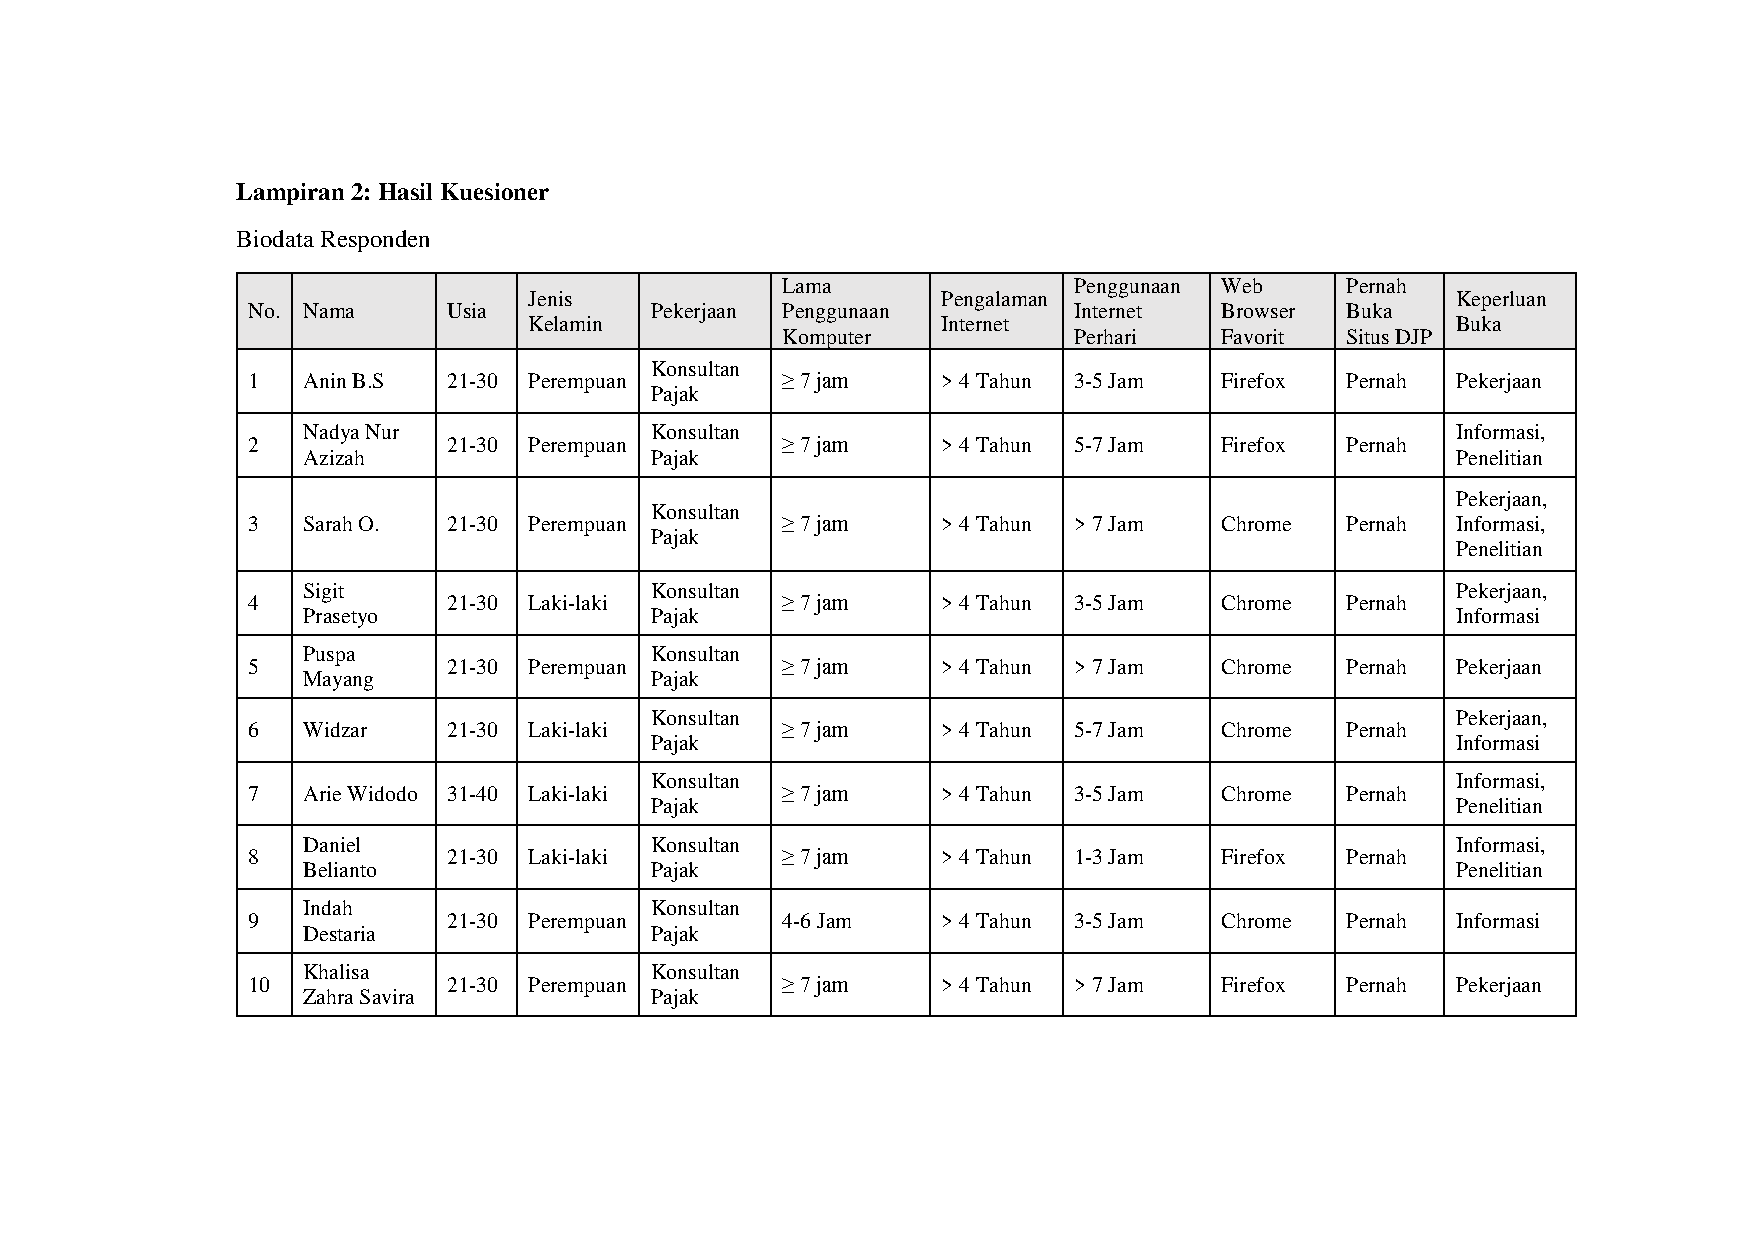
\includepdf[pagecommand={}, pages={-},fitpaper,landscape=true]{pics/rekapdokumen}

\end{landscape}
%-----------------------------------------------------------------------------%
\addChapter{Lampiran 3 : Izin Penelitian DJP}
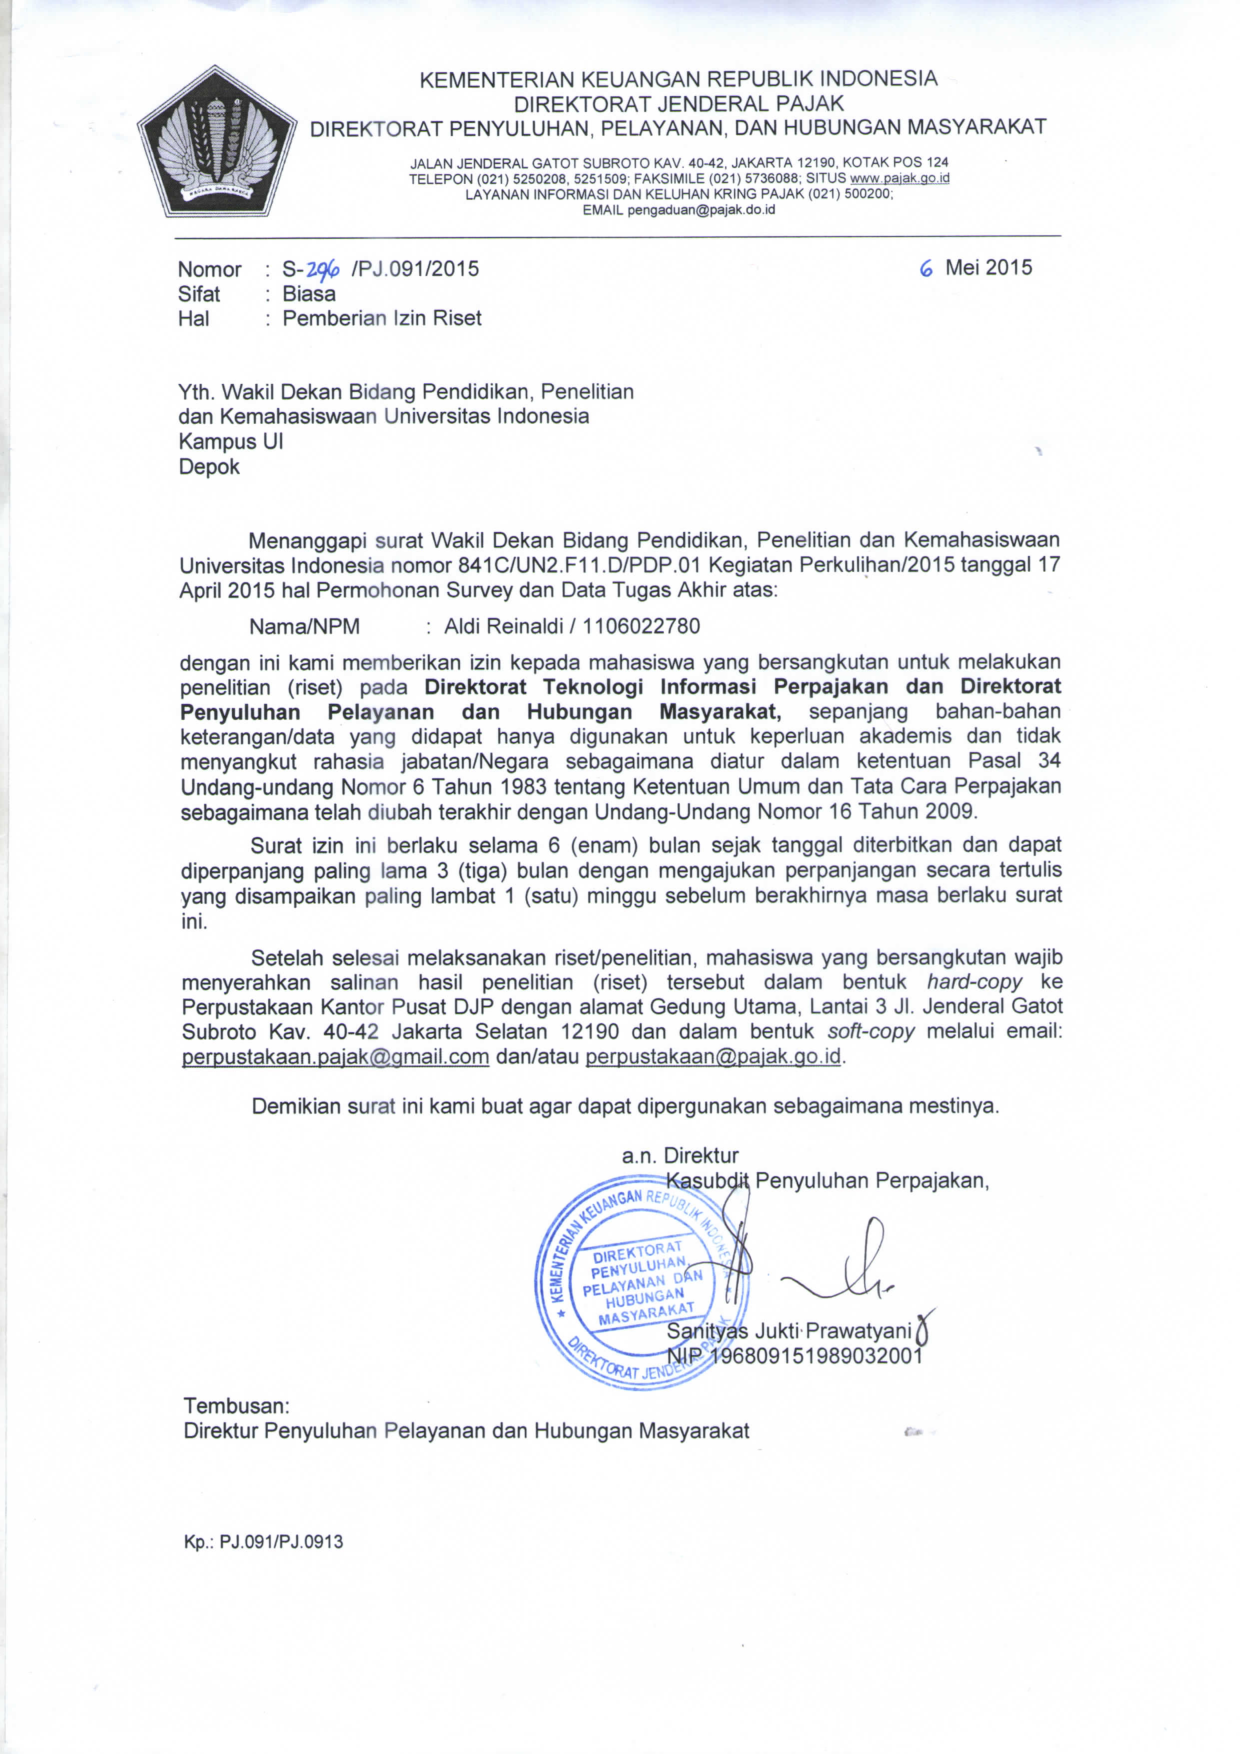
\includepdf[pagecommand={}, pages={-}, fitpaper]{pics/suratdjp.pdf}
%-----------------------------------------------------------------------------%



\end{appendix}

\end{document}